
%% bare_jrnl.tex
%% V1.4b
%% 2015/08/26
%% by Michael Shell
%% see http://www.michaelshell.org/
%% for current contact information.
%%
%% This is a skeleton file demonstrating the use of IEEEtran.cls
%% (requires IEEEtran.cls version 1.8b or later) with an IEEE
%% journal paper.
%%
%% Support sites:
%% http://www.michaelshell.org/tex/ieeetran/
%% http://www.ctan.org/pkg/ieeetran
%% and
%% http://www.ieee.org/

%%*************************************************************************
%% Legal Notice:
%% This code is offered as-is without any warranty either expressed or
%% implied; without even the implied warranty of MERCHANTABILITY or
%% FITNESS FOR A PARTICULAR PURPOSE!
%% User assumes all risk.
%% In no event shall the IEEE or any contributor to this code be liable for
%% any damages or losses, including, but not limited to, incidental,
%% consequential, or any other damages, resulting from the use or misuse
%% of any information contained here.
%%
%% All comments are the opinions of their respective authors and are not
%% necessarily endorsed by the IEEE.
%%
%% This work is distributed under the LaTeX Project Public License (LPPL)
%% ( http://www.latex-project.org/ ) version 1.3, and may be freely used,
%% distributed and modified. A copy of the LPPL, version 1.3, is included
%% in the base LaTeX documentation of all distributions of LaTeX released
%% 2003/12/01 or later.
%% Retain all contribution notices and credits.
%% ** Modified files should be clearly indicated as such, including  **
%% ** renaming them and changing author support contact information. **
%%*************************************************************************


% *** Authors should verify (and, if needed, correct) their LaTeX system  ***
% *** with the testflow diagnostic prior to trusting their LaTeX platform ***
% *** with production work. The IEEE's font choices and paper sizes can   ***
% *** trigger bugs that do not appear when using other class files.       ***                          ***
% The testflow support page is at:
% http://www.michaelshell.org/tex/testflow/



\documentclass[journal,10pt]{IEEEtran}
%
% If IEEEtran.cls has not been installed into the LaTeX system files,
% manually specify the path to it like:
% \documentclass[journal]{../sty/IEEEtran}





% Some very useful LaTeX packages include:
% (uncomment the ones you want to load)


% *** MISC UTILITY PACKAGES ***
%
%\usepackage{ifpdf}
% Heiko Oberdiek's ifpdf.sty is very useful if you need conditional
% compilation based on whether the output is pdf or dvi.
% usage:
% \ifpdf
%   % pdf code
% \else
%   % dvi code
% \fi
% The latest version of ifpdf.sty can be obtained from:
% http://www.ctan.org/pkg/ifpdf
% Also, note that IEEEtran.cls V1.7 and later provides a builtin
% \ifCLASSINFOpdf conditional that works the same way.
% When switching from latex to pdflatex and vice-versa, the compiler may
% have to be run twice to clear warning/error messages.






% *** CITATION PACKAGES ***
%
%\usepackage{cite}
% cite.sty was written by Donald Arseneau
% V1.6 and later of IEEEtran pre-defines the format of the cite.sty package
% \cite{} output to follow that of the IEEE. Loading the cite package will
% result in citation numbers being automatically sorted and properly
% "compressed/ranged". e.g., [1], [9], [2], [7], [5], [6] without using
% cite.sty will become [1], [2], [5]--[7], [9] using cite.sty. cite.sty's
% \cite will automatically add leading space, if needed. Use cite.sty's
% noadjust option (cite.sty V3.8 and later) if you want to turn this off
% such as if a citation ever needs to be enclosed in parenthesis.
% cite.sty is already installed on most LaTeX systems. Be sure and use
% version 5.0 (2009-03-20) and later if using hyperref.sty.
% The latest version can be obtained at:
% http://www.ctan.org/pkg/cite
% The documentation is contained in the cite.sty file itself.






% *** GRAPHICS RELATED PACKAGES ***
%
\ifCLASSINFOpdf
  % \usepackage[pdftex]{graphicx}
  % declare the path(s) where your graphic files are
  % \graphicspath{{../pdf/}{../jpeg/}}
  % and their extensions so you won't have to specify these with
  % every instance of \includegraphics
  % \DeclareGraphicsExtensions{.pdf,.jpeg,.png}
\else
  % or other class option (dvipsone, dvipdf, if not using dvips). graphicx
  % will default to the driver specified in the system graphics.cfg if no
  % driver is specified.
  % \usepackage[dvips]{graphicx}
  % declare the path(s) where your graphic files are
  % \graphicspath{{../eps/}}
  % and their extensions so you won't have to specify these with
  % every instance of \includegraphics
  % \DeclareGraphicsExtensions{.eps}
\fi


% correct bad hyphenation here
\hyphenation{op-tical net-works semi-conduc-tor}
\let\chapter\section
\usepackage{amsmath}
\newtheorem{thm}{Theorem}
\newtheorem{prop}[thm]{Proposition}
\allowdisplaybreaks[4]
\usepackage{graphicx}
\usepackage{caption}
\usepackage{subfigure}
\usepackage{multirow}
\usepackage{caption}
\usepackage{amssymb}
\usepackage{chngpage}
\usepackage{array}
%\usepackage{algorithm}
%\usepackage{algorithmic}
\usepackage[ruled,boxed,linesnumbered]{algorithm2e}
%\usepackage{hyperref}
\usepackage{bm}
\usepackage{mathrsfs}
\usepackage{leftidx}
\usepackage{authblk}
\usepackage{booktabs}
\usepackage{tabularx}
\usepackage{threeparttable}
\usepackage[square, comma, sort&compress, numbers]{natbib}
\captionsetup{font={small}}
\usepackage{color}
\setcounter{secnumdepth}{3}
\usepackage{setspace}
\usepackage{float}
\newcommand*{\TitleFont}{%
      %\usefont{\encodingdefault}{\rmdefault}{b}{n}%
      \fontsize{22}{27.5}%
      \selectfont}
\usepackage{natbib}
\begin{document}

% paper title
% Titles are generally capitalized except for words such as a, an, and, as,
% at, but, by, for, in, nor, of, on, or, the, to and up, which are usually
% not capitalized unless they are the first or last word of the title.
% Linebreaks \\ can be used within to get better formatting as desired.
% Do not put math or special symbols in the title.
\title{\TitleFont Joint Power-Rate-Slot Resource Allocation in Energy Harvesting-Powered Wireless Body Area Networks}
%Energy-aware Resource Allocation in EH-powered D2D Communications underlaying Cellular Networks}
%Efficient Resource Allocation in Energy-Harvesting powered D2D Communications underlay Cellular Networks: A Space Matching approach
%
%
% author names and IEEE memberships
% note positions of commas and nonbreaking spaces ( ~ ) LaTeX will not break
% a structure at a ~ so this keeps an author's name from being broken across
% two lines.
% use \thanks{} to gain access to the first footnote area
% a separate \thanks must be used for each paragraph as LaTeX2e's \thanks
% was not built to handle multiple paragraphs
%

\author{Zhiqiang~Liu,~\IEEEmembership{Student Member, IEEE},
        Bin~Liu,~\IEEEmembership{Member, IEEE},
        and~Chang~Wen~Chen,~\IEEEmembership{Fellow,~IEEE}% <-this % stops a space
\thanks{Zhiqiang Liu is with the Key Laboratory of Electromagnetic Space Information, Chinese Academy of Sciences, Department of Electrical Engineering and Information Science, University of Science and Technology of China, Hefei 230027, China (e-mail: lzhq28@mail.ustc.edu.cn).}% <-this % stops a space
\thanks{Bin Liu is with the Key Laboratory of Electromagnetic Space Information, Chinese Academy of Sciences, School of Information and Technology, University of Science and Technology of China, Hefei 230027, China (e-mail: flowice@ustc.edu.cn).}
\thanks{Chang Wen Chen is with Department of Computer Science and Engineering, University at Buffalo, State University of New York, New York 002837, USA (e-mail: chencw@buffalo.edu).}}






% make the title area
\maketitle
 
% As a general rule, do not put math, special symbols or citations
% in the abstract or keywords.
\begin{abstract}
 
Wireless body area network (WBAN) has become a promising network for continuous health monitoring of various diseases. 
The limited energy of sensors in WBAN cannot support the long-term work with the high requirements of Quality of Service (QoS) for health applications. 
Energy harvesting (EH)-powered WBAN, which can provide uninterrupted work, has attracted more attention from both academic and industry. 
However, the time-varying and heterogeneous EH states of different sensors become an important factor when designing the resource allocation schemes in EH-powered WBAN.
In this paper, we propose a novel two-phase resource allocation scheme, which optimizes the allocation of the transmission power, the source rate and the time slots to improve the QoS performances of EH-powered WBAN. 
In the first phase, we investigate the statistical knowledge of energy harvesting to measure the long-term QoS performances, and then a joint Power-Rate Control Scheme (PRCS) is proposed to optimize the transmission power and the source rate for ensuring the long-term QoS performance.
Moreover, we design a QoS Aware Slot Allocation Scheme (QASAS) to dynamically adjust the time slot allocation to cope with the time-varying and heterogeneous EH states for obtaining better short-term QoS performances in the second phase.
Finally, numerical simulation results demonstrate that the proposed joint Power-Rate-Slot Resource Allocation scheme (PRS-RA) of EH-powered WBANs can efficiently exploit the time-varying EH to improve both the long-term and short-term QoS performances.
 
\end{abstract}

% Note that keywords are not normally used for peerreview papers.
\begin{IEEEkeywords}
 energy harvesting, resource allocation, wireless body area network (WBAN).
\end{IEEEkeywords}



\IEEEpeerreviewmaketitle
\section{Introduction}
With the rapid development of sensors and wireless communication technologies, wireless body area network (WBAN) can replace complex and wired healthcare applications to monitor the body's vital signals continuously and provide real-time feedback to the users and doctors without causing any discomfort and interrupting their daily lifestyle \cite{salayma2017wireless,movassaghi2014wireless,dagdeviren2017energy}. 
WBAN typically consists of several low-power, miniaturized and lightweight on-body or implanted sensor nodes to monitor physiological parameters. These collected physiological data are further transmitted to the remote medical servers by one energy-efficient hub (Mobile phone or PDA) for various medical and healthcare applications \cite{zhang2017medium}. 
Most of these applications are related to the chronic diseases, which need to continuously monitor the body's vital signals without interrupting user's daily lifestyle. Besides, for carrying out an adequate diagnosis, the Quality of Service (QoS) should be guaranteed in terms of packet loss, delay and so on \cite{razzaque2017qos}. 

However, the limited battery capacity, constrained by the size and weight of sensors nodes, cannot support the long-term operation without interruption. And replacing the battery or taking off sensors to charge power is not always practical especially for some implanted sensors, which also causes the interruption of the health monitoring system \cite{ibarra2016qos,luo2017resource}. Although the traditional energy-saving technologies make efforts to explore different energy efficient schemes in aspects of the MAC protocol design, the power control schemes and the cross-layer resource scheduling strategies to prolong the system lifetime \cite{zhang2017medium,zang2016accelerometer,liu2017transmission}, the ultimate goal 'uninterrupted work' cannot be ensured. 
Fortunately, the energy harvesting (EH) technology, which can collect energy from various sources around the human body, has recently been considered as a promising solution to overcome the bottleneck of energy limited WBANs \cite{hao2017energy}. For instance, EH-powered sensors can scavenge energy from a variety of ambient sources (e.g., light, heat, electromagnetic radiation) or the body itself (e.g., locomotion, breathing, heartbeat, lactate), and then convert it to usable electric energy for providing continuous power \cite{akhtar2017energy}. 
Sensors can also combine several types of EH sources for acquiring more energy to support more strict QoS requirements \cite{ibarra2016qos}.
Therefore, EH-powered WBANs have the potential ability to achieve an infinite lifetime and perpetual operation, which is called Energy Neutral Operation (ENO) \cite{kansal2007power}.
In the literature, researchers have paid more and more attention on how to keep in ENO state with considering the QoS performances in EH-powered WBANs.

Most of the researchers investigated the statistical characteristics of the energy harvesting in the resource allocation schemes to support the long-term QoS performances \cite{ibarra2016qos,ozel2011transmission,leng2017resource}. 
However, due to the dynamic ambient or body conditions, the EH states are time-variant and different for each node.
The allocated resources for supporting the long-term QoS performances may not cope with the dynamic demand of the sensors due to the time-varying EH states, and then the short-term QoS performances cannot be fully guaranteed.
Therefore, the time-varying EH states can be exploited to allocate the resources for improving the short-term QoS performances dynamically. This phenomenon will lead to a important result: the time-varying and heterogeneous EH states become a significant factor in designing the effective resource allocation scheme for improving both the long-term and short-term QoS performances. 

\subsection{Related works}
Compared with EH-powered wireless sensor networks (WSNs), the human body contains more bio-energy sources besides the ambient source for various kinds of energy harvesters in WBANs \cite{leng2017resource}. These bio-energy sources can be classified into biochemical and biomechnical energy sources. The biochemical energy sources convert electrochemical reactions to electricity for implanted body sensors, while the harvesters can scavenge energy from the voluntary and involuntary actions of the human body as biomechnical energy sources \cite{akhtar2017energy}. The scavenged energy can be converted to electric potential by appropriated harvesters, and then stored in a rechargeable battery or a super-capacitor for powering up wireless body sensors \cite{wahbah2014characterization}. The energy harvesting efficiency can be improved to harvest more energy through the elaborate hardware circuit design \cite{xia20140,el201610}. Therefore, the available power density by collecting energy from human body gradually reaches the $\mu W$ range, which can run low-power-consuming wireless devices, such as Bluetooth4.0 \cite{bluetooth2010}, MicaZ \cite{kramer2006energy}, MultiMode \cite{wong20131} and so on. However, the harvesting process of human body sensors is unstable and time-varying due to the dynamic body movement status \cite{hao2017energy}. Thus, the time-varying EH states should be taken full consideration in the resource allocation schemes.

In the literature, some researchers have focused on the resource allocation schemes for EH-powered WBANs. These resource allocation schemes can be divided into two categories in terms of the priori knowledge of the channel state, data state and energy state for the transmitter: the offline schemes \cite{mosavat2017maximizing,varan2016delay,shan2015discrete,tutuncuoglu2012optimum,wei2015power,huang2014optimal} and the online schemes \cite{leng2017resource,ibarra2016qos,alhawari2016power,dionisi2016autonomous,shaviv2016universally,liu2015optimal,ozel2011transmission}. 
For the offline schemes, it is assumed that the transmitter has the perfect priori knowledge of the channel state, the data state and the energy state when it allocates the resources. 
In \cite{tutuncuoglu2012optimum}, the short-term throughput and the transmission completion time were regarded as the objective function to obtain the optimum power allocation with a deadline constraint and finite energy storage capacity, while energy arrivals were assumed as a priori known. 
Shan \textsl{et al.} \cite{shan2015discrete} proposed a general framework to transform a continuous-rate model into practical discrete transmission rates with keeping the optimality. The per-application quality-of-service (QoS) could be guaranteed by the optimal rate scheduling algorithm for an EH enabled transmitter, assuming that the information regarding packets and harvesting was known in advance. 
Varan \textsl{et al.} \cite{varan2016delay} considered the throughput maximization problem with finite energy and data storage constraints, and new notions of water pumps and overflow bins were added to the directional water-filling for solving the energy scheduling problem.  
In addition, the weighted sum of the outage probabilities was the objective function to be minimized in the power control policy, while the harvested energy was known as a priori to the scheduler, and a near-optimal offline scheme was designed with only high signal-to-noise ratios due to the non-convex objective function \cite{wei2015power,huang2014optimal}.
The above offline resource allocation schemes commonly construct the convex optimization problems and analytical solutions to obtain the optimal resource allocation results with the perfect non-causal and priori knowledge. Therefore, the offline schemes can only serve as a benchmark of the resource allocation schemes, or the EH states are predictable for some stable energy sources.   

Compared with the offline schemes, only the causal information and statistical knowledge of energy states, data states, and channel states can be utilized in the online schemes to manage the data packets and the collected energy. 
Ozel \textsl{et al.} \cite{ozel2011transmission} maximized the number of bits sent by a deadline given only the distributions of the energy arrivals and channel fade levels. 
Leng and Yener \cite{leng2017resource} maximized the long-term expected throughput under the energy constraints, and the close-form expression of optimal transmission power was obtained by formulating the Lagrangian and solving the KKT conditions.
However, the long-term throughput maximization problem only allocates the resources from the statistical characteristics of EH states. The time-varying EH states, which have a significant effect on the transmissions of packets, are not mentioned. 
Liu \textsl{et al.} \cite{liu2015optimal} modeled the transmission power and time allocation optimization problem as a Markov decision process (MDP) to provide a sustainable and high-quality service for EH-powered WBAN. 
However, MDP based resource allocation schemes have a high complexity for wireless devices with limited computational capabilities in WBANs, and they are highly dependent on the accuracy models of channel fading level, energy arrivals and data arrivals, which are hardly obtained in practice. 
To achieve the best possible QoS performances, the authors of \cite{ibarra2016qos} proposed a joint power-QoS control scheme for making optimal use of harvested energy to efficiently transmit the respective data packets of only one sensor in WBAN. However, the channel fading was not considered in the scheme, which could not deal with the dynamic link characteristics in WBANs. In addition, the time-varying and heterogeneous EH states of different body sensors were not adequately considered.

\subsection{Contributions}
In this paper, we take the time-varying and heterogeneous EH states into consideration and develop an efficient resource allocation scheme for EH-powered WBANs to support both the long-term and short-term QoS requirements.
The important contributions of this paper are expressed as three aspects:
 \begin{enumerate}
	 \item As far as we know, this work is the first to combine the transmission power, source rate and time slots to effectively allocate the resources under dynamic link characteristics of heterogeneous body sensors. The time-varying EH states are regarded as an essential factor to reallocate the resources for coping with the variation of the harvesting available energy.
Hence, the harvested energy can be efficiently utilized to improve both the long-term and short-term QoS performances.
	 \item For supporting the long-term QoS performances of body sensors, we design a power-rate control scheme to optimize the transmission power and the source rates for different body sensors, subject to the long-term QoS requirements under the Energy Neutral Operation (ENO).
The statistical knowledge of energy harvesting and channel fading is investigated to measure the QoS performances with the allocated resources. Then, an optimal numerical solution is successfully obtained through the transformation of the non-convex problem. 
	\item To further improve the short-term QoS performances and the resource utilization, we propose a QoS aware slot allocation scheme to dynamically adjust the time slot allocation based on the states of each sensor for better transmitting data packets.
The time-varying and heterogeneous EH states, which causes the fluctuation of the available energy and the data queues, are carefully studied. Then the energy states and the queue states are evaluated and adopted to predict the states of each sensor. 
Finally, the QoS aware slot allocation scheme can give a timely response to the changes of the sensor state to improve the short-term QoS performances.

 \end{enumerate}
The remainder of this paper is organized as follows. 
In Section \ref{sec:system_model}, the system model is presented. In Section \ref{sec:PRCS}, a joint power-rate optimization allocation problem is formulated and solved to optimally allocate the transmission powers and the source rates for each sensor. 
In Section \ref{sec:QASAS}, the sensor states are evaluated based on the energy state and queue buffer state, and a short-term QoS aware slot allocation scheme is provided in details.
In Section \ref{sec:simulation}, the numerical results are discussed and analyzed. Finally, Section \ref{sec:conclusion} concludes the paper.

\section{System model} \label{sec:system_model}
In this section, we give the details of the node's architecture and the WBAN topology in EH-based WBAN. Then, the energy harvesting model is introduced. Finally, the energy consumption model is correspondingly obtained with the dynamic link characteristics.

\subsection{Node's Architecture and WBAN Topology}
We consider a classical WBAN which consists of one hub and $N$ EH-powered wireless sensor nodes. 
Suppose that the hub (such as a PDA and a mobile phone) has sufficient resources to implement some resource allocation scheme with a high computation complexity, and the wireless sensor nodes placed in different positions of the body have limited processing and storage resources with energy harvesters. The set of body sensor nodes is expressed as $\mathcal{C}_{node}=\left\{1,2,\cdots,N \right\}$. As recommended by IEEE 802.15.6 \cite{ieee2012WBAN}, the body sensor nodes collect the vital signals and communicate directly with the hub, and a star topology is adopted with considering the constrained resources of sensor nodes. In addition, a scheduled access mechanism in beacon mode with superframe boundaries is adopted to access the channel without collisions, idle listening and overhearing of sensor nodes for saving scarce energy. One superframe is formed by one beacon and $M$ slots, and the set of slots are expressed as $\mathcal{C}_{slot}=\left\{1,2,...,M\right\}$. In the beacon of a superframe, the hub broadcasts the beacon packets to configure the transmission rates, source rates and dedicate time slots for each node. The sensor node only turns active in its dedicate time slots to transmit data signals, and turns sleep in other slots for saving energy. In each node, the vital signals are collected and packetized in the data queue, which will be transmitted to the hub with the First-In-First-Out (FIFO) queue strategy and the retransmission strategy \cite{liu2017buffer}. Thus, the packet losses only occur in two situations: the data queue overflow and the delay over the preset threshold. 

\subsection{Energy Harvesting Model}
\begin{figure}[!htb]
\centering
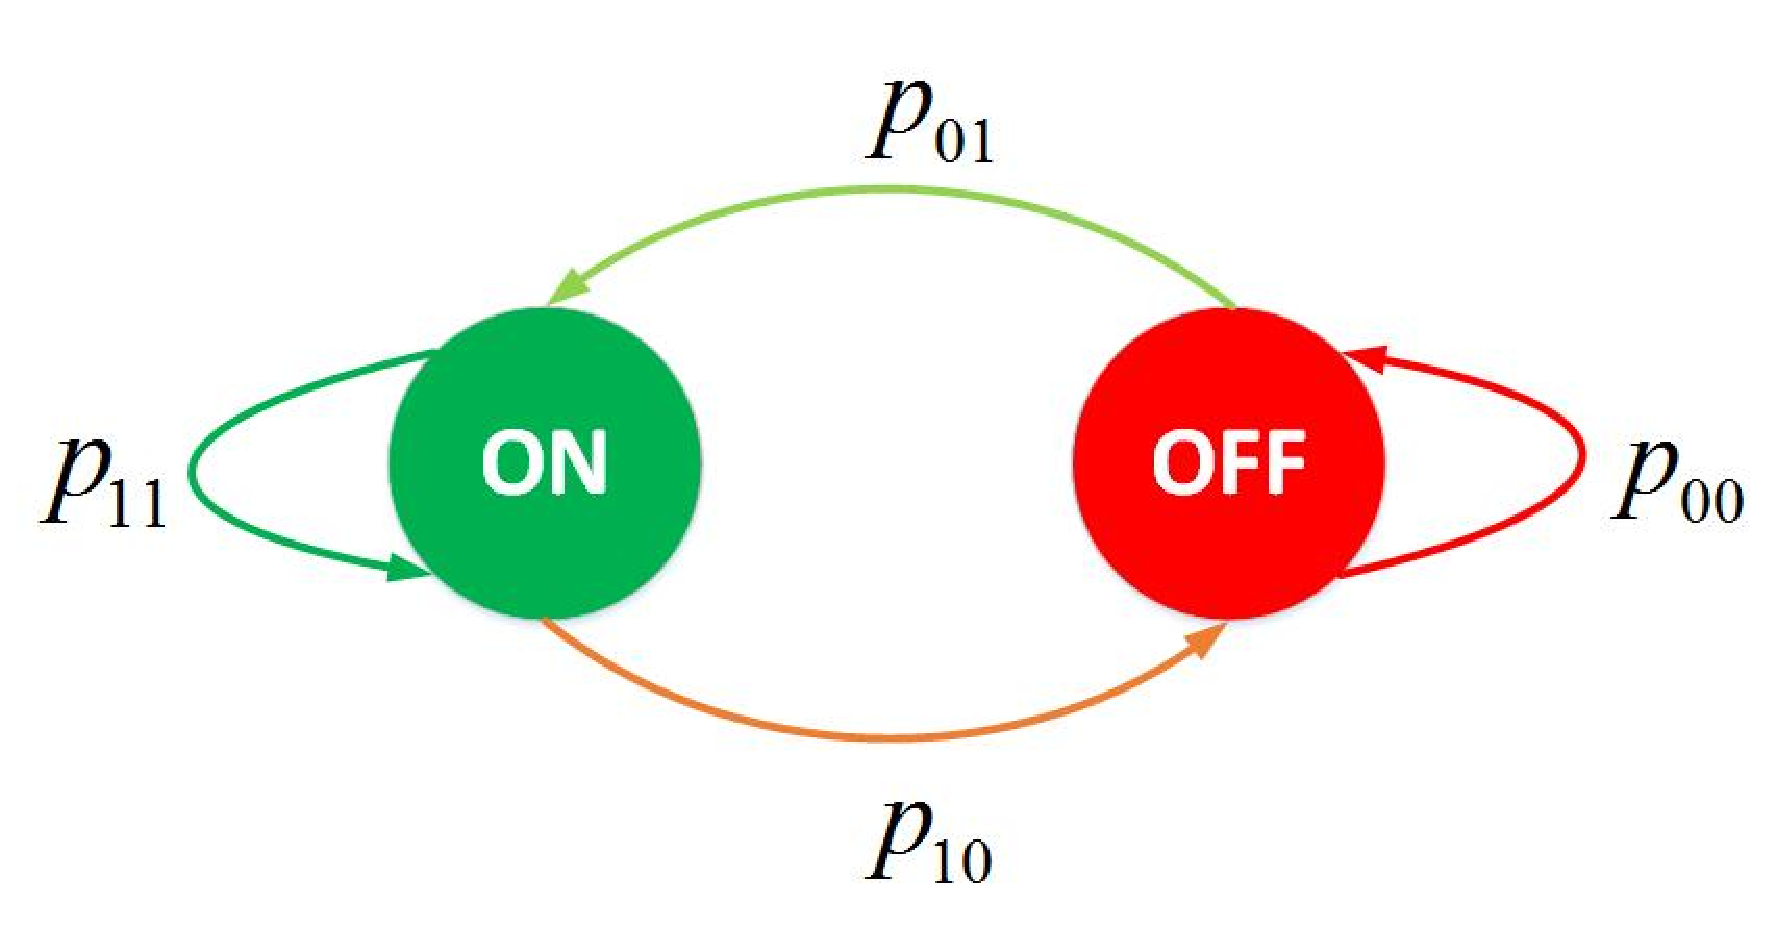
\includegraphics[width=0.3\textwidth]{markov_model}
\caption{Discrete Two-state Markov Chain of the EH process}
\label{fig:markov_model}
\end{figure}

In this paper, the harvested energy is stored in a rechargeable battery or a super-capacitor, and then used to power the body sensor node \cite{akhtar2017energy}. 
The EH process of each node can be modeled as a correlated discrete-time Markov chain with two states: the active state (ON) and the inactive state (OFF) \cite{seyedi2010energy,ibarra2016qos}.
In the ON state, it means the ambient or body conditions are conducive to generate the energy by the energy harvester (i.e. when the intensity of the motion can produce disturbances in the transducer to harvest energy). In the OFF state, the energy harvester does not collect any energy. 
In addition, the coherence time of the EH process is set to $t_{cor}=k \cdot  t_{slot}$, where $t_{slot}$ is the time length of one time slot in the superframe. We assume that the energy acquisition rate $\rho $ in the ON state follows an uniform distribution in range of $[EH_{min}, EH_{max}]$, which is based on the conditions of energy sources. 
Due to the different positions and functions of different sensor nodes, the adopted energy harvesters may collect energy from different energy sources. 
For instance, the sensor node on the foot can utilize the piezoelectric transducer to harvest energy from the body motion \cite{geisler2017human}, and the sensor node for capturing the electrocardiograph (ECG) signal may use a thermoelectric generator to harvest from the body temperature \cite{thielen2017human}. Therefore, the EH states of different nodes are heterogeneous, and the energy acquisition rate in the ON state is different for different sensor nodes.
The Markov chain of EH process is shown in Fig. \ref{fig:markov_model}. $p_{01}$ means the transition probability from the OFF state to the ON state, while $p_{10}$ represents the transition probability from the ON state to the OFF state. The probability of keeping the ON state and the OFF state are regarded as $p_{11}=1-p_{10}$ and $p_{00}=1-p_{01}$, respectively. And the steady probabilities of the ON state and the OFF state are expressed as follows, 
\begin{equation}
{\mu _{on}} = {{{p_{01}}} \over {{p_{01}} + {p_{10}}}}
\end{equation}
\begin{equation}
{\mu _{off}} = {{{p_{10}}} \over {{p_{01}} + {p_{10}}}}
\end{equation}

\subsection{Energy Consumption Model}
In body sensor nodes, most of the energy is consumed to transmit data packets and receive ACK packets, while the energy consumption of the processing and beacon listening can be ignored \cite{xiao2009transmission}. The transmission energy consumption mainly consists of two parts: the transmit amplifier energy consumption $E_{tx}$ and the circuitry energy consumption $E_{ct}$ \cite{he2011optimal,liu2017buffer}. Thus, the energy model of transmitting packets can be expressed as follows,
\begin{equation}
E_{tran} = \left( {1 + \alpha } \right){E_{tx}} + {E_{ct}}
\end{equation}

Compared with the energy consumption of transmitting packets, the energy model of receiving packets only contains the circuitry energy consumption $E_{ct}$.
\begin{equation}
E_{rec} = {E_{ct}}
\end{equation}
where $\alpha$ means the power amplifier inefficiency factor, $E_{tx}=P_{tx}t$ and $E_{ct}=P_{ct}t$. $P_{tx}$ represents the transmission power of the transmitter. $P_{ct}$ is the circuitry power, which is a constant depending on the specific transmitter \cite{lin2009asymmetric}. 

To improve the QoS performances, the transmission power should be dynamically adjusted to cope with the time-varying link quality. Thus, the path loss model of wireless links becomes an important factor for the energy consumption. In this paper, the path loss model $PL\left( d \right)$ for both Light-Of-Sight (LOS) and None-Light-Of-Sight (NLOS) scenarios follows the log normal distribution as recommended by the IEEE 802.15.6 \cite{ieee2012WBAN}.
\begin{equation}\label{eq:PL}
\small{
PL\left( d \right) ={PL_{d_0}} + 10n{\log _{10}}\left( {\frac{d}{{{d_0}}}} \right) + {X_\sigma }
}
\end{equation}
where $PL_{d_0}$ is the path loss at the referent distance $d_0$, and $n$ represents the path-loss exponent. The shadowing $X_\sigma$ follows the normal distribution $\mathcal{N}\left( {\mu_{s},\sigma_{s}^2 } \right)$, and the statistic characteristics are related to the human postures and the environments \cite{reusens2009characterization}\cite{d2010statistical}. 

\section{Long-term Power-Rate Control Scheme} \label{sec:PRCS}
In this section, the throughput maximization problem is designed to maximize total throughput with the time-varying EH states, subject to the long-term QoS constraints. Then, the optimal numerical solution is given to solve the optimization problem efficiently through the convex transformation. Finally, the source rate is allocated based on the optimal throughput results with considering both the effective diagnosis and the energy saving.

 
\subsection{Throughput Maximization Problem}
The QoS requirements should be guaranteed for the effective diagnostic when designing the resource allocation scheme. Considering the dynamic link characteristics, the exact link quality cannot be known as a priori in the online scheme. In this paper, the average PLR performance is regarded as the main long-term QoS constraint. With the statistic knowledge of the path loss model, the average PLR can be derived through the following equations.
Firstly, the PLR can be expressed as the function of the bit Signal to Noise Ratio (bit SNR),
\begin{equation}
PLR({\gamma }) = 1 - {\left( {1 - {P_{b,B}}({\gamma })} \right)^L}
\end{equation}
where bit SNR can be calculated as ${\gamma } =  {10^{\frac{{{P_{tx,dB}} - PL\left( d \right) - {P_{N}}}}{{10}}}} \frac{B}{R}$. $L$ is the length of a packet in bits. $P_{tx,dB}$ is the transmission power in dB. $P_{N}$ is the power of noise. $B$ represents the system bandwidth. $P_{b,B}$ indicates the equivalent bit error rate based on the modulation and the channel coding \cite{goldsmith2005wireless}. 

Then, the average PLR is the mean value over the range of bit SNR with its probability density function. It can be calculated as the following equation,
\begin{equation} \footnotesize
\overline{PLR}  = \int\limits_0^{ + \infty } {PLR({\gamma})} P({\gamma}|{\mu _{{\gamma _{dB}}}},{\sigma _{{\gamma _{dB}}}})d{\gamma }
\end{equation}
where $P({\gamma}|{\mu _{{\gamma _{dB}}}},{\sigma _{{\gamma _{dB}}}})$ represents the probability density function of bit SNR $\gamma$, and it follows a log-normal distribution as the shadowing $X_{\sigma}$. $\mu _{{\gamma _{dB}}}$ and ${\sigma _{{\gamma _{dB}}}}$ are the mean and the standard deviation of $\gamma$ in dB, respectively. 

Finally, the long-term QoS constraint can be depicted that the average PLR should be less than the preset threshold as follows,
\begin{equation}  \small
\overline{PLR} < PLR_{th}
\end{equation}
where $PLR_{th}$ is the preset threshold of the packet loss rate.

As we all know, the larger transmission power could result in better QoS performances, but the achievable throughput is lower due to the larger energy cost per bit. Not only the long-term PLR performance but also the achievable throughput should be taken into consideration. The energy acquisition rate of the energy harvester decides how much energy can be collected to transmit data packets. 
Considering the time-varying and heterogeneous EH states, the available harvesting energy changes over time. Therefore, the achievable throughput is constrained by both the QoS performances and the EH states. 
In this paper, we optimize the allocation of the transmission power to maximize the throughput, subject to the long-term PLR performance and the EH states. The throughput maximization problem can be constructed as follows,

\begin{subequations}\label{P1:PRCS} \small
\begin{align}
    \textbf{P1:}& \qquad\mathop {\max }\limits_{\small{({P_{tx,i},{\upsilon_i}})}} \; {\sum\limits_{i = 1}^{N} {{\upsilon_i}} } , \label{P1:obj} \\
    s.t.\quad %&{\sum\limits_{i = 1}^{i \in {\cal N}} {{S_i}}  \cdot T \le R \cdot T}, \label{P1:con1} \\
		& {\rm{0}} \le {{{\upsilon_i}} \over {1 - PL{R_{i,th}}}},\label{P1:con1}\\
    & {{{\upsilon_i}} \over {1 - PL{R_{i,th}}}} \le {{{{\mu _{on}} \cdot R \cdot \overline{EH_{i}} } \over {\left[ {\left( {1 + \alpha } \right){P_{tx,i}} + {P_{ct,i}}} \right]}}},\label{P1:con2}\\
    & {\overline {PL{R_i}}  \le PL{R_{i,th}}},\label{P1:con3}\\
    & {{P_{tx,\min }} \le {P_{tx,i}} \le {P_{tx,\max }}}, \label{P1:con4}
\end{align}
\end{subequations}
where ${\upsilon_i}$ represents the throughput for node $i$, and $PLR_{i,th}$ is the threshold of the packet loss rate for node $i$.
$\overline{EH_{i}} ={{{\left( {E{H_{i,\max }} + E{H_{i,\min }}} \right)} \mathord{\left/
 {\vphantom {{\left( {E{H_{i,\max }} + E{H_{i,\min }}} \right)} {\rm{2}}}} \right.
 \kern-\nulldelimiterspace} {\rm{2}}}}$ is the mean of the energy harvesting rate for node $i$.
 $\overline {PL{R_i}}$ represents the average packet loss rate with the allocation transmission power $P_{i}$. $P_{tx,min}$ and $P_{tx,max}$ are the minimum value and the maximum value of the transmission power for the transmitter. We assume all the nodes have the same type transmitter for the sake of simplicity.

With respect to \textbf{P1}, the objective function (\ref{P1:obj}) is to maximize the total throughput under the long-term QoS constraints. The constraint (\ref{P1:con1}) means the throughput should be no less than zero. The average collected energy by the energy harvester can be evaluated by exploring the statistical characterizations of the EH states. Then, the equivalent throughput with considering PLR has an upper boundary which just uses the average collected energy as expressed in constraint (\ref{P1:con2}). In constraint (\ref{P1:con3}), the allocated transmission power should guarantee the long-term average PLR performance. Equation (\ref{P1:con4}) means the allocated transmission power should be in the range of $[P_{tx,min},P_{tx,max}]$.

\subsection{Optimal Numerical Solution}

The above optimization problem \textbf{P1} is a nonlinear and non-convex problem, and it is difficult to be solved. Fortunately, we find that the optimization problem \textbf{P1} is very similar to the form of the Geometric Program (GP), which can be solved efficiently and reliably \cite{boyd2004convex}. Here, we try best to transform the problem \textbf{P1} into the form of the Geometric Program (GP).

Obviously the objective function (\ref{P1:obj}) is a posynomial function. All constraints, expect (\ref{P1:con2}) and (\ref{P1:con3}), can be easily converted to the form of a posynomial less than or equal to one. Fortunately, both constraints (\ref{P1:con2}) and (\ref{P1:con3}) can be successfully transformed into the form of posynomial inequalities through the following methods.

Firstly, even though the PLR constraint (\ref{P1:con3}) does not have an analytical expression, we have proved that the average PLR constraint is the monotone function of bit SNR in \cite{liu2017transmission}. Hence, the PLR constraint can be equivalent to the constraint of the mean of bit SNR as follows, 

\begin{equation}
{\mu _{{\gamma _{dB}}}} \ge \mu_{th}
\end{equation}
where $\mu_{th}$ just satisfies the equation \resizebox{0.3\hsize}{!}{$\overline {PLR\left( {{\mu _{{th}}}} \right)}=PLR_{th}$}. And ${\mu _{{\gamma _{dB}}}}= E\left[ {10{{\log }_{10}}\left( {\frac{B}{R}} \right) + {P_{tx,dB}} - {PL\left( d \right)}- {P_{N}}} \right]$. Then, the equivalent PLR constraint can be expressed as follows,
\begin{equation} 
\begin{split}
P_{tx}{R^{{ - 1}}} & \ge {B^{ - 1}} {10^{\frac{{\mu _{th}+ {PL_{d_0}} + 10n{\log _{10}}\left( {\frac{d}{{{d_0}}}} \right)  + {P_{N}}}}{{10}}}} = {\theta _{th}}
\end{split}
\end{equation} 

Then, a new intermediate variable is defined as ${\xi_i} = {1 \over { {\left( {1 + \alpha } \right){P_{tx,i}} + {P_{ct,i}}} }}$ to transform the constraint (\ref{P1:con2}). The optimization problem \textbf{P1} is finally transformed to the form of the Geometric Program (GP), as shown in follows,

\begin{subequations}\label{P2:PRCS} \small
\begin{align}
    \textbf{P2:}& \qquad\mathop {\max }\limits_{\small{({{\xi_i},{\upsilon_i}})}} \; {\sum\limits_{i = 1}^{ N} {{\upsilon_i}} } , \label{P2:obj} \\
    s.t.\quad %&{\sum\limits_{i = 1}^{i \in {\cal N}} {{\upsilon_i}}  \cdot T \le R \cdot T}, \label{P2:con1} \\
		& {\rm{0}} \le {{{\upsilon_i}} \over {1 - PL{R_{i,th}}}},\label{P2:con1}\\
    & {{{{\upsilon_i} \cdot \xi_i^{ - 1}} \over {1 - PL{R_{i,th}}}} \le {\mu _{on}} \cdot R \cdot \overline{EH_{i}} },\label{P2:con2}\\
    & {{\xi_i} \le {1 \over {{P_{ct,i}} + \left( {1 + \alpha } \right) \cdot {\theta _{th}} \cdot R}}},\label{P2:con3}\\
    & {1 \over {\left( {1 + \alpha } \right) \cdot {P_{tx,\max }} + {P_{ct,i}}}}  \le {\xi_i} , \label{P2:con4} \\
		& {\xi_i} \le {1 \over {\left( {1 + \alpha } \right) \cdot {P_{tx,\min }} + {P_{ct,i}}}}, \label{P2:con5}
\end{align}
\end{subequations}

Finally, the throughput maximization problem \textbf{P2} as a classical GP can be solved efficiently by many custom solvers. Then, the optimal transmission power $P_{tx,i}^{*}, i \in \mathcal{C}_{node} $ and the corresponding achievable throughput $\upsilon_i^{*}, i \in \mathcal{C}_{node} $ can be obtained.

\subsection{Source Rate Configuration}
The optimal throughput for each node can be obtained through solving the throughput maximization problem with the time-varying EH states. The source rates for each node can be configured according to the optimal achievable throughput. 
In addition, different applications have different requirements of the source rates for satisfying the effective diagnosis. 
For vital signals, the larger source rate means more useful information can be used for diagnosis, and the larger source rate will cost more energy to be transmitted. 
The limited energy and dynamic link quality will result in many packet losses with an exorbitant source rate, and the random packet losses will break the integrity of data. Therefore, the source rate usually has a most appropriate upper boundary $S_{up}$ of the source rate, which contains enough information for diagnosis.
In addition, the source rate also has a acceptable low boundary $S_{low}$. If the source rate is lower than the low boundary $S_{low}$, the vital data will lose the diagnostic significance. 
Therefore, the boundaries of the source rate as well as the optimal achievable throughput jointly determine the configuration value of the source rate as follows,

\begin{equation}
S_{i} = \max \left\{ \min (\upsilon_{i}^{*}, S_{up,i} ), S_{low,i} \right\}
\end{equation}

When the optimal achievable throughput $\upsilon^{*}$ is larger than the upper boundary $S_{up}$, it means the harvesting energy is enough for supporting the source rate $S_{up}$. Meanwhile, the long-term PLR performance is also satisfied by solving the maximization problem \textbf{P2}. 
Then, the source rate is set to the upper boundary $S_{up}$ for fair diagnosis and energy efficiency. 
When the throughput $\upsilon^{*}$ is in the range of $[S_{low},S_{up}]$, the source rate is set to the optimal throughput $\upsilon^{*}$ to just meet the throughput requirements for keeping more details of the data signals. Otherwise, the source rate is configured as the low boundary $S_{low}$ to ensure the diagnostic significance.
However, the throughput condition cannot be satisfied with current energy harvesting rate, and there will be packets blocked in the data queue. Fortunately, the problem can be solved by the proposed short-term QoS aware resource allocation scheme in the following section.


\section{Short-term QoS Aware Slot Allocation Scheme} \label{sec:QASAS}
In the above section, the long-term QoS performances are considered with the time-varying EH states from statistical analysis. However, the time-varying EH states and dynamic link quality may cause the fluctuations of the data queue. In this section, we explore the time slot allocation to further improve the short-term QoS performances. Firstly, we analyze the energy harvesting process in details. Then, the sensor state evaluation method is given. Finally, the different slot allocation schemes are adopted for nodes with different states.

\subsection{Energy Harvesting Process Analysis}
For better allocating slots for each node, the time-varying and heterogeneous EH states should be carefully studied to adjust the allocation of slots.
As we adopt the scheduled access mechanism in beacon mode with superframe boundaries, nodes only turn active in its dedicated slots to transmit the data packets while keeping sleep for saving energy in other slots. 
Because the EH states of each node in a superframe are different, the collected energy by each node is also different.
For instance, if the EH state of one node has a high probability to keep the OFF state at the beginning of the following superframe, it means the slots at the end of the following superframe can be allocated to the node for collecting more energy with more harvesting time.
In this paper, only the EH states of nodes in the allocated slots of the last superframe can be known by the hub, thus the EH states of each sensor in the following superframe need to be predicted for better allocating the slots.
The energy harvesting process is modeled as a two-state Markov chain as shown in Fig. \ref{fig:markov_model}. The transition matrix can be expressed as follows,
\begin{equation}
{\rm \textbf{P}} = \left[ {
\begin{matrix}
   {1 - {p_{01}}} & {{p_{01}}}  \cr 
   {{p_{10}}} & {1 - {p_{10}}}  \cr 
\end{matrix} 
 } \right]
\end{equation}

We define the probability of EH state to be the ON state in a $x$-th slot is denoted by $p(x)$. After $\tau$ slots, the EH state has been transferred ${\left\lceil\frac{\tau}{k}\right\rceil}$ times. ${\lceil \cdot \rceil}$ is the ceiling function.
The probability of the ON state after $\tau$ slots can be calculated as follows \cite{tselishchev2011reducing},
\begin{equation} \footnotesize \label{eq:P_ON_1}
\begin{split}
p(x+\tau) &= \left[\begin{matrix}
		1 - p(k) & p(k)
  \end{matrix}\right] 
	\cdot \textbf{P}^{\left\lceil\frac{\tau}{k}\right\rceil} \cdot
	\left[\begin{matrix}
		0\\
		1
  \end{matrix}\right]  \\
  &= {{{p_{01}}} \over Q}+ {{p\left( k \right) \cdot {p_{10}} - \left( {{\rm{1}} - p\left( k \right)} \right) \cdot {p_{01}}} \over Q} \cdot {\left( {1 - Q} \right)^{\left\lceil {{\tau  \over k}} \right\rceil }}
\end{split}
\end{equation} 
where $Q = {p_{01}} + {p_{10}}$. Suppose the EH state in the $x$-th slot is known, then the probability of the ON state $p(x)$ is equal to 0 when the EH state is OFF. Otherwise $p(x)$ is set to 1 with the ON state. Thus, the Eq. \eqref{eq:P_ON_1} can be expressed as,
\begin{equation} \label{eq:P_ON_2}
p(x+\tau) =\left\{ { \begin{array}{l}
{{{{{p_{01}}} \over Q} - {{{p_{01}}\cdot{{\left( {1 - Q} \right)}^{\left\lceil\frac{\tau}{k}\right\rceil} }} \over Q},{\rm{  }}p\left( {x } \right) = 0}}\\
{{{{{p_{01}}} \over Q} + {{{p_{10}}\cdot{{\left( {1 - Q} \right)}^{\left\lceil\frac{\tau}{k}\right\rceil} }} \over Q},{\rm{  }}p\left( {x } \right) = 1}}
\end{array}}\right.
\end{equation}

The EH states of each node in the following superframe can be predicted, while the last EH state in the allocated slot of the last superframe can be obtained through the feedback from the node.

\subsection{Sensor State Evaluation}
Due to the heterogeneous EH states, the residual energy from energy harvesters is different in different nodes. Besides, the number of packets for each node in the data queue is also time-varying. 
If the blocked packets are not timely transmitted to the hub, the QoS performances of both the blocked packets and the arriving packets will be degraded by adopting the First-In-First-Out (FIFO) queue strategy. 
Hence, the slot allocation should be according to both the energy level in the energy buffer and the predicted EH states for further improving the short-term QoS performances. When the residual energy is sufficient to transmit the arriving packets in the following superframe, the number of slots for the blocked packets should be taken into consideration for timely transmission to decrease the short-term packet delay. 
Otherwise, the residual energy is constrained, and the number of allocated slots is only allocated for the arriving packets to ensure the throughput of the queue model. The blocked packets will be transmitted until the residual energy is sufficient with high EH acquisition rate.
Thus, the sensor states for each node are evaluated before allocating slots.

For the energy-sufficient nodes, the amount of the harvesting energy in the following superframe is not necessary, while they are insensitive to the location of allocated slots in the following superframe. 
Therefore, the number of allocated slots becomes important to transmit both the arriving data packets and the blocked packets in the data queue. 
As for the energy-constrained nodes, the locations of the allocated slots need to be carefully adjusted to harvest more energy based on their EH states. In addition, the number of the allocated slots is at least enough to transmit the arriving packets for satisfying the throughput condition.
Thus, the nodes can be classified into two categories based on the residual energy: the energy-sufficient nodes and the energy-constrained nodes.
\begin{equation} \label{eq:energy_con}
 \textbf{Con1:} \quad {E_{res,i}} \ge \left[ {\left( {1 + \alpha } \right){P_{tx,i}} + {P_{ct,i}}} \right] \cdot {{{S_i} \cdot T} \over R}
\end{equation}
where $E_{res,i}$ denotes the residual energy in node $i$. When the above condition \eqref{eq:energy_con} is satisfied for sensor $i$, the node $i$ belongs to the GOOD node set ${\Phi _{GOOD}}$. Otherwise, the node $i$ belongs to the BAD node set ${\Phi _{BAD}}$.

The nodes in ${\Phi _{BAD}}$, which are sensitive to the locations of allocated slots, should be firstly allocated for the time slots. If there are several energy-constrained nodes in ${\Phi _{BAD}}$, the locations of slots are allocated based on their predicted EH states in the following superframe.
Then, the rest of the nodes are allocated for these nodes in ${\Phi _{GOOD}}$ with considering both the arriving packets and the blocked packets in the data queue.
\begin{equation} \small
Node_{i} \in \left\{ { \begin{array}{l}
\begin{aligned}
{\Phi _{GOOD}} &, \text{  If \textbf{Con1} is satisfied.} \\
{\Phi _{BAD}} &, \text{ Otherwise}
\end{aligned}
\end{array}}\right. , \forall i \in \mathcal{C}_{node}
\end{equation}


\subsection{Slot Allocation Scheme for Energy-Constrained Nodes}
\begin{figure}[!htb]
\centering
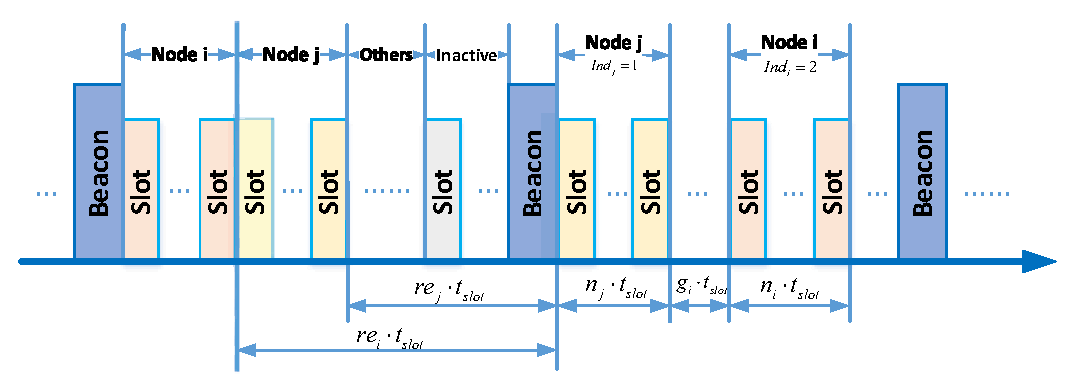
\includegraphics[width=0.5\textwidth]{slot_allocation}
\caption{Details of slot allocations for each sensor.}
\label{fig:slot_allocation}
\end{figure}


%For the energy-constrained nodes in the BAD set ${\Phi _{BAD}}$, the residual energy is limited to transmit the arriving data in the next framework. Thus, it should harvest more energy before its dedicated slot in the following framework. 

Generally, the node with the allocated slot at the end of the superframe will have more time to collect energy.
Due to the time-varying and heterogeneous EH states for nodes, there may be several nodes in the BAD set ${\Phi _{BAD}}$. Hence, we should study their arriving energy in the following superframe based on the predicted EH states, and then dynamically allocate the slots for these nodes in ${\Phi _{BAD}}$ with considering both the number and the locations.

Firstly, we evaluate how long each sensor will take to harvest enough energy to transmit the arriving packets through calculating the arriving energy with the predicted state in the following superframe. The probability of the ON state in the last allocated slot can be obtained by the hub through the feedback from the node $i$, which is regarded as $p_{i}(0)$. Then, the probability of the ON state for the following slots can be predicted as the equation \eqref{eq:P_ON_2}. 
Thus, the total harvesting energy after $m$ slots on average from the last allocated slot is calculated as follows,
\begin{equation}  
F_{i,EH}(m) = {\sum\limits_{l = 1}^m {\left( {{p_i}\left( {r{e_i} + l} \right) \cdot \overline {E{H_i}}  \cdot {t_{slot}}} \right)} }
\end{equation}
where $re_{i}$ is the number of slots from the last allocated slot to the current beacon as shown in Fig. \ref{fig:slot_allocation}. Obviously, the function $F_{i,EH}(m)$ is a monotone function of time. 
Therefore, the required number of slots after the current beacon, called the expected waiting time $\eta_{i}$ for node $i$, can be obtained to harvest enough energy to transmit the arriving data as the following equation,
\begin{equation} \small
\eta_{i} = \mathop {\arg }\limits_m \left\{ { F_{i,EH}(m)   = \left[ {\left( {1 + \alpha } \right){P_{tx,i}} + {P_{ct,i}}} \right] \cdot {{{S_i} \cdot T} \over R}} \right\}
\end{equation}

For different nodes in ${\Phi _{BAD}}$, the node with the larger expected waiting time $\eta$ means that it needs more time to harvest energy before the next transmissions. It should be allocated the slots after the nodes with the smaller expected waiting time $\eta$.
Thus the expected waiting time $\eta$ is used to sort the nodes for allocating slots in this paper.

After ordering the nodes, the slot allocation consists of two aspects: the number of slots and the locations of slots. As shown in Fig.~\ref{fig:slot_allocation}, the specific allocated slots for sensor $i$ can be determined by two parameters: $g_{i}$ and $n_{i}$. $g_{i}$ represents the number of slots between the end of allocated slots for previous node and the begin of allocated slots for node $i$, while $n_{i}$ denotes the number of allocated slots for node $i$. 
Finally, the slot allocation problem can be stated as: to maximize the difference between the location and the expected waiting time of all nodes for achieving more energy for these energy-constrained nodes by optimizing the number and the locations of slots for each sensor. Mathematically, the problem can be formulated as follows,
\begin{subequations} \label{P3:slot_allocation}
\begin{align}
    \textbf{P3:}& \quad \mathop {\max }\limits_{\small{({g_{i},{n_i}})}} \;  {G_{sum}}\left(\eta_{i},{g_{i},{n_i}} \right), \label{P3:obj} \\
    s.t.\quad & {\sum\limits_{i \in {\Phi _{BAD}}} {\left( {{g_i} + {n_i}} \right) } \le M} , \label{P3:con1} \\
		& R \cdot {n_i} \cdot {t_{slot}} \ge D_{i},\label{P3:con2}\\
    & {{g_i},{n_i} \in {\Bbb N}}, i \in {\Phi _{BAD}}, \label{P3:con3}
\end{align}
\end{subequations}
where ${G_{sum}}$ is the sum distance between the location and the expected waiting time of all nodes as the objective function, which can be expressed as follows,
\begin{equation}\label{math:sum_gain}
\begin{array}{l}
    {G_{sum}}\left(\eta_{i},{g_{i},{n_i}} \right) = \\
    \quad {\sum\limits_{i \in {\Phi _{BAD}}} {\left( {\sum\limits_{\left\{ {j \in {\Phi _{BAD}}|{\eta _j} < {\eta _i}} \right\}} {\left( {{g_j} + {n_j}} \right) + {g_i} - {\eta _i}} } \right)} }.
\end{array}
\end{equation}

In the constraint (\ref{P3:con1}), the number of allocated slots should be less than the total number $M$ of slots in a superframe. As for the constraint (\ref{P3:con2}), the number of allocated slots for each sensor should be able to transmit the arriving data with considering the packet loss rate, where the equivalent arriving data $D_{i}$ for node $i$ can be expressed as follows,
\begin{equation}
D_{i}={{{S_i} \cdot \left( {r{e_i} + \sum\limits_{\left\{ {j \in {\Phi _{BAD}}|{\eta _j} \le {\eta _i}} \right\}} {\left( {{g_j} + {n_j}} \right)} } \right) \cdot {t_{slot}}} \over {\left( {1 - PL{R_{i,th}}} \right)}}
\end{equation}

The slot allocation problem \textbf{P3} is an Integer Linear Programming (ILP), which can be solved efficiently \cite{boyd2004convex}. After allocating slots for the energy-constrained nodes, the remaining slots are then assigned to the energy-sufficient nodes in the GOOD set ${\Phi _{GOOD}}$.

\subsection{Slot Allocation Scheme for Energy-Sufficient Nodes}

Compared with the energy-constrained nodes, the energy-sufficient nodes have enough energy to transmit the arriving data, and they are insensitive to the locations of allocated slots. 
Considering the time-varying EH states, some data packets may be blocked in the data queue with the dynamic link quality. If the blocked data packets cannot be transmitted to the hub, they will lead to the increasing delay of not only the blocked packets but also the arriving packets \cite{liu2017buffer}. Therefore, the blocked data packets in the data queue need to be transmitted for improving the short-term QoS performances, when there is sufficient residual energy in the energy buffer. 

Considering both the blocked data ${D_{block}}$ in the data queue and the arriving data in the following superframe, the total data ${D_{buf}}$ can be expressed as follows,
\begin{equation}
{D_{buf,i}} = {D_{block,i}} + {S_i} \cdot T
\end{equation}

The remaining number of slots ${N_{rest}}$ after the slot allocation for energy-constrained nodes can be calculated as follows,
\begin{equation}
{{N_{rest}} = M - \sum\limits_{i \in {\Phi _{BAD}}} {{n_i}}}
\end{equation}

Thus, the total number of the allocated slots for the energy-sufficient nodes should be not larger than the remaining number of slots ${N_{rest}}$, given as follows,

\begin{equation}
\sum\limits_{i \in {\Phi _{GOOD}}}^{} {{n_i} \leqslant {N_{rest}}}
\end{equation}

For different energy-sufficient nodes, they expect to be allocated enough slots for transmitting both the blocked data and the arriving data. However, there should be enough energy for supporting the transmission in the energy buffer, as satisfying the following constraint,
\begin{equation}
{{E_{res,i}} + \overline {E{H_i}}  \cdot T \geqslant \left[ {\left( {1 + \alpha } \right){P_{tx,i}} + {P_{ct,i}}} \right] \cdot {n_i} \cdot {t_{slot}}}
\end{equation}

To evaluate the satisfaction of both the blocked data and the arriving data with given number of slots, a utility function $U(m,D_{buf})$ is defined as follows,  

\begin{equation} \label{eq:utility}  \footnotesize
U(m,D_{buf}) = \frac{{\left( {{(R\cdot m \cdot t_{slot})^2} - 2 \cdot (R\cdot m \cdot t_{slot}) \cdot D_{buf}  } \right)}}{{D_{buf}^2}}
\end{equation}

When the number of allocated slots is less than $\frac{D_{buf}}{R \cdot t_{slot}}$, which just supports the transmissions of both the blocked packets and the arriving packets,  more allocated slots can achieve a higher utility to transmit more data in the queue buffer. When the number of the allocated slots reaches the value $\frac{D_{buf}}{R \cdot t_{slot}}$, the node obtains the highest utility with the highest bandwidth utilization. If still increasing the number of allocated slots, part of allocated slots will not be used. Thus, it will cause the decreasing of the bandwidth utilization, and the utility will decrease correspondingly.
Finally, the slot allocation problem for the energy-sufficient nodes can be formulated to maximize the total utility of all nodes in the GOOD set, subject to the total slot constraint and the energy constraint. Mathematically, the slot optimization problem can be written as follows,

\begin{subequations} \label{P4:slot_allocation} \small
\begin{align}
    \textbf{P4:}& \quad \mathop {\max }\limits_{\small{({{n_i}})}} \;  \sum\limits_{i \in {\Phi _{GOOD}}} {U\left( {{n_i} ,{D_{buf,i}}} \right)} , \label{P4:obj} \\
    s.t.\quad & {\sum\limits_{i \in {\Phi _{GOOD}}}^{} {{n_i} \leqslant {N_{rest}}}} , \label{P4:con1} \\
		& {{E_{res,i}} + \overline {E{H_i}}  \cdot T \geqslant \left[ {\left( {1 + \alpha } \right){P_{tx,i}} + {P_{ct,i}}} \right] \cdot {n_i} \cdot {t_{slot}}},\label{P4:con2}\\
    & {{n_i} \in {\Bbb N}}, i \in {\Phi _{GOOD}}, \label{P4:con3}
\end{align}
\end{subequations}

With respect to \textbf{P4}, the problem is a classical Quadratic Problem (QP), which can also be solved efficiently with using many custom solvers \cite{lofberg2004yalmip}.

\section{Simulation results} \label{sec:simulation}
In this section, we investigate the performance of the proposed joint Power-Rate-Slot resource allocation scheme in terms of average PLR, packet delay, throughput and energy efficiency.
To evaluate the effectiveness of the proposed algorithms, there are two comparison schemes: the offline scheme \cite{huang2014optimal} and the online scheme \cite{ibarra2016qos}.
Due to the lack of the IEEE 802.15.6-based hardware, we develop an event-driven WBAN system in the MATLAB. A MATLAB-based optimization toolbox, YALMIP \cite{lofberg2004yalmip}, is embedded in the simulation environment to solve the proposed optimization problems. To better simulate the channel, the channel reference code by IEEE 802.15.6 standard \cite{yazdandoost2009channel} is adopted as the channel module in the WBAN system.

\subsection{Simulation Setup}
%Above all, the WBAN simulation settings should be illustrated in details. 
In this paper, we consider a classical WBAN system, which contains one hub and $N=5$ wireless body nodes. The deployed positions and link parameters of all nodes are given in Table \ref{tab:posNode}, referring to the actual link experiment results in \cite{d2010statistical} \cite{reusens2009characterization}. The changes of postures are modeled as a Markov chain, and we only consider three most common postures, i.e., still, walking and running with 0.5, 0.3 and 0.2 steady-state probabilities, correspondingly. We assume the hub can identify the changes of postures with high accuracy in real-time \cite{guo2016two}. The extension to more body postures is straightforward. 
The standard derivation $\sigma_{s}$ of the shadowing changes with the postures. The mean of the shadowing is used to indicate the quality of the environment, and the larger mean of the shadowing represents the bad channel environment \cite{d2010statistical}. 
In this paper, we assume the hub has sufficient energy supply, while the body nodes are powered by a piezoelectric energy harvester according to the intensity of postures. Besides, the energy harvesting rates of different body nodes are heterogeneous with considering the different intensity of body parts, which also change with the postures, as well as the steady-state probabilities of the EH states \cite{ibarra2016qos}, as shown in Table \ref{tab:parEH}. Other parameters are summarized in Table \ref{tab:otherPar} according to the IEEE 802.15.6 specifications \cite{ieee2012WBAN}. 

\begin{table} \scriptsize
\setlength{\abovecaptionskip}{-2pt}
\setlength{\belowcaptionskip}{0pt}
\caption{Parameters of body nodes for different postures}
\begin{center}
\begin{tabular}{|c|c|c|c|c|c|c|c|c|} \hline
\multicolumn{1}{|c}{} & \multicolumn{3}{c|}{}&\multicolumn{3}{c|}{${\sigma _{{S}}}{(dB)}$}& \multicolumn{2}{c|}{\scriptsize{\textbf{Data Rate}(Kbps)}}\\ \hline
 \textbf{Index} & \textbf{${d}$} & \textbf{${n}$}&\textbf{${PL_{d_{0}}}$}&\scriptsize{\textbf{Still}}  & \scriptsize{\textbf{Walk}}  & \scriptsize{\textbf{Run}}    & ${S_{up}}$ &${S_{low}}$ \\ \hline \hline
1   & 69 &3.11&35.2&6.1   &	5.4	&  5.7   &  40 & 20\\  \hline
2   & 36 &3.23&41.2& 4.8	&    7.4	&    7.8   & 68& 30\\  \hline
3   & 48 &3.35&32.2& 5.1	&     4.9&    4.5    & 34 & 16  \\  \hline
4   & 34 &3.45&32.5& 2.6	&    4.4	&    4.0    & 50 & 25\\  \hline
5   & 100 &3.11&35.2& 2.2	&    3.6	&    2.6   &  35 & 16\\  \hline
\end{tabular}
\end{center}
\label{tab:posNode}
\end{table}


\begin{table*}  \scriptsize
\setlength{\abovecaptionskip}{-2pt}
\setlength{\belowcaptionskip}{0pt}
\caption{Parameters of energy harvesters}
\begin{center}
\begin{tabular}{|c|c|c|c|c|c|c|c|c|c|} \hline
&\multicolumn{3}{c|}{\textbf{Still (mW)}}&\multicolumn{3}{c|}{\textbf{Walking (mW)}}& \multicolumn{3}{c|}{\textbf{Running (mW)}}\\ \hline
\textbf{Node index}&$EH_{min}$&$EH_{max}$&${\mu _{on}}$&$EH_{min}$&$EH_{max}$&${\mu _{on}}$& $EH_{min}$&$EH_{max}$&${\mu _{on}}$\\ \hline 
1   &	 0.01 &0.015&0.9& 	 0.04 &	0.05	&  0.3    &  0.06 & 0.07 & 0.4\\  \hline
2   & 0.02 &0.025&0.8&  	0.06  &	0.07	&  0.4  	 &  0.09 & 0.11 & 0.5\\  \hline
3   & 0.015 &0.02&0.9&  	 0.035  &	0.05	&  0.3  	 &  0.04 & 0.06 & 0.45\\  \hline
4   & 0.03 &0.04&0.8&  	0.055  &	 0.06	&  0.4   	&  0.07 & 0.08 & 0.6\\  \hline
5   & 0.02 &0.03&0.7&  	0.08  &	0.10	&  0.6   	&  0.09 & 0.11 & 0.8\\  \hline
\end{tabular}
\end{center}
\label{tab:parEH}
\end{table*}


\begin{table}[h]
\footnotesize
\centering
\caption{EH-powered WBAN simulation parameters}
 \begin{tabular}{|m{0.12\columnwidth}<{\centering}| m{0.4\columnwidth}<{\centering}| m{0.23\columnwidth}<{\centering}|}
  \hline
  \textbf{{Parameter}} & {\textbf{Description}} & {\textbf{Value}}  \\
  \hline
   $B$ & bandwidth & 1MHz \\
  \hline
   $P_{N}$ & noise power & -94dBm \\
  \hline
   $\alpha$ & power amplifier inefficiency & 2.4 \\
  \hline
   $E_{ct}$ & circuitry energy consumption & 50uW \\
  \hline
   $t_{slot}$ &  time length of one time slot  & 0.5ms \\
		   \hline
   $M$ &  number of slots in one superframe  & 200 \\
	  \hline
   $R$ &  transmission rate  & 485.6kbps \\
	   \hline
   $P_{tx,min}$ &  minimum value of the transmission power  & -30dBm \\
	   \hline
   $P_{tx,max}$ &  maximum value of the transmission power  & 0dBm \\
   \hline
   $PLR_{th}$ &  preset threshold of the packet loss rate  & 5\% \\
   \hline
   $Delay_{th}$ &  preset threshold of the packet delay  & 500ms \\
   \hline
   $D_{buf}$ &  packet buffer size  & 100kb \\

  \hline
  %\bottomrule
 \end{tabular}
\label{tab:otherPar}
\end{table}





\subsection{The Effectiveness of Long-term Power-Rate Control Scheme}

Firstly, we analyze the allocated results of the long-term power-rate control scheme (PRCS) for different postures. As shown in Table \ref{tab:posNode}, the parameters of the path loss are different to different nodes as well as the source rate, and the statistical characterizations of the shadowing fluctuate for different postures.
Therefore, the resource allocation schemes should be able to deal with the dynamic link quality. 
The allocated transmission power and source rates for different nodes by the proposed PRCS in different postures are given in Fig. \ref{fig:PRCS}. 
In the PRCS, we optimize the transmission power for each node based on the link quality to support the long-term QoS performances. The allocated transmission powers for each node are dynamically adjusted when the link quality changes due to the postures in Fig. \ref{fig:PRCS_power}. For instance, the node 3 and the node 4 are close to the hub, and their link qualities are much better than the other nodes. Hence, the transmission powers for them are assigned a lower value to save precious energy under the condition of satisfying the long-term QoS requirements. 

In addition, the source rates for different nodes are adjusted based on the heterogeneous requirements and the energy harvesting rates. As shown in Fig. \ref{fig:PRCS_rate}, the source rates of the node 1 and the node 2 are allocated as the low boundary $S_{low}$ in all postures. 
This is because the achievable throughput $\upsilon^{*}$ with the highest energy harvesting rates of them still does not reach the low boundary $S_{low}$ in Fig. \ref{fig:PRCS_power}. 
As for node 5, the energy harvesting rates in different postures are different for the piezoelectric energy harvester in Table \ref{tab:parEH}. In still posture, the achievable throughput $\upsilon^{*}$ is lower than the low boundary $S_{low}$, thus the source rate is allocated as the low boundary $S_{low}$ to support the diagnostic significance. In walking posture, the source rate is allocated as the achievable throughput $\upsilon^{*}$, which is in the range of $[S_{low},S_{up}]$. In running posture, the energy harvesting rate can support the upper boundary of the source rate $S_{up}$, then the source rate is set to the upper boundary $S_{up}$ for saving energy.
Thus, the source rates are adjusted based on the achievable throughput with the corresponding energy harvesting rate. 

\begin{figure}[!htb]
\centering
    \subfigure[Allocated transmission power by PRCS]{
        \label{fig:PRCS_power}
        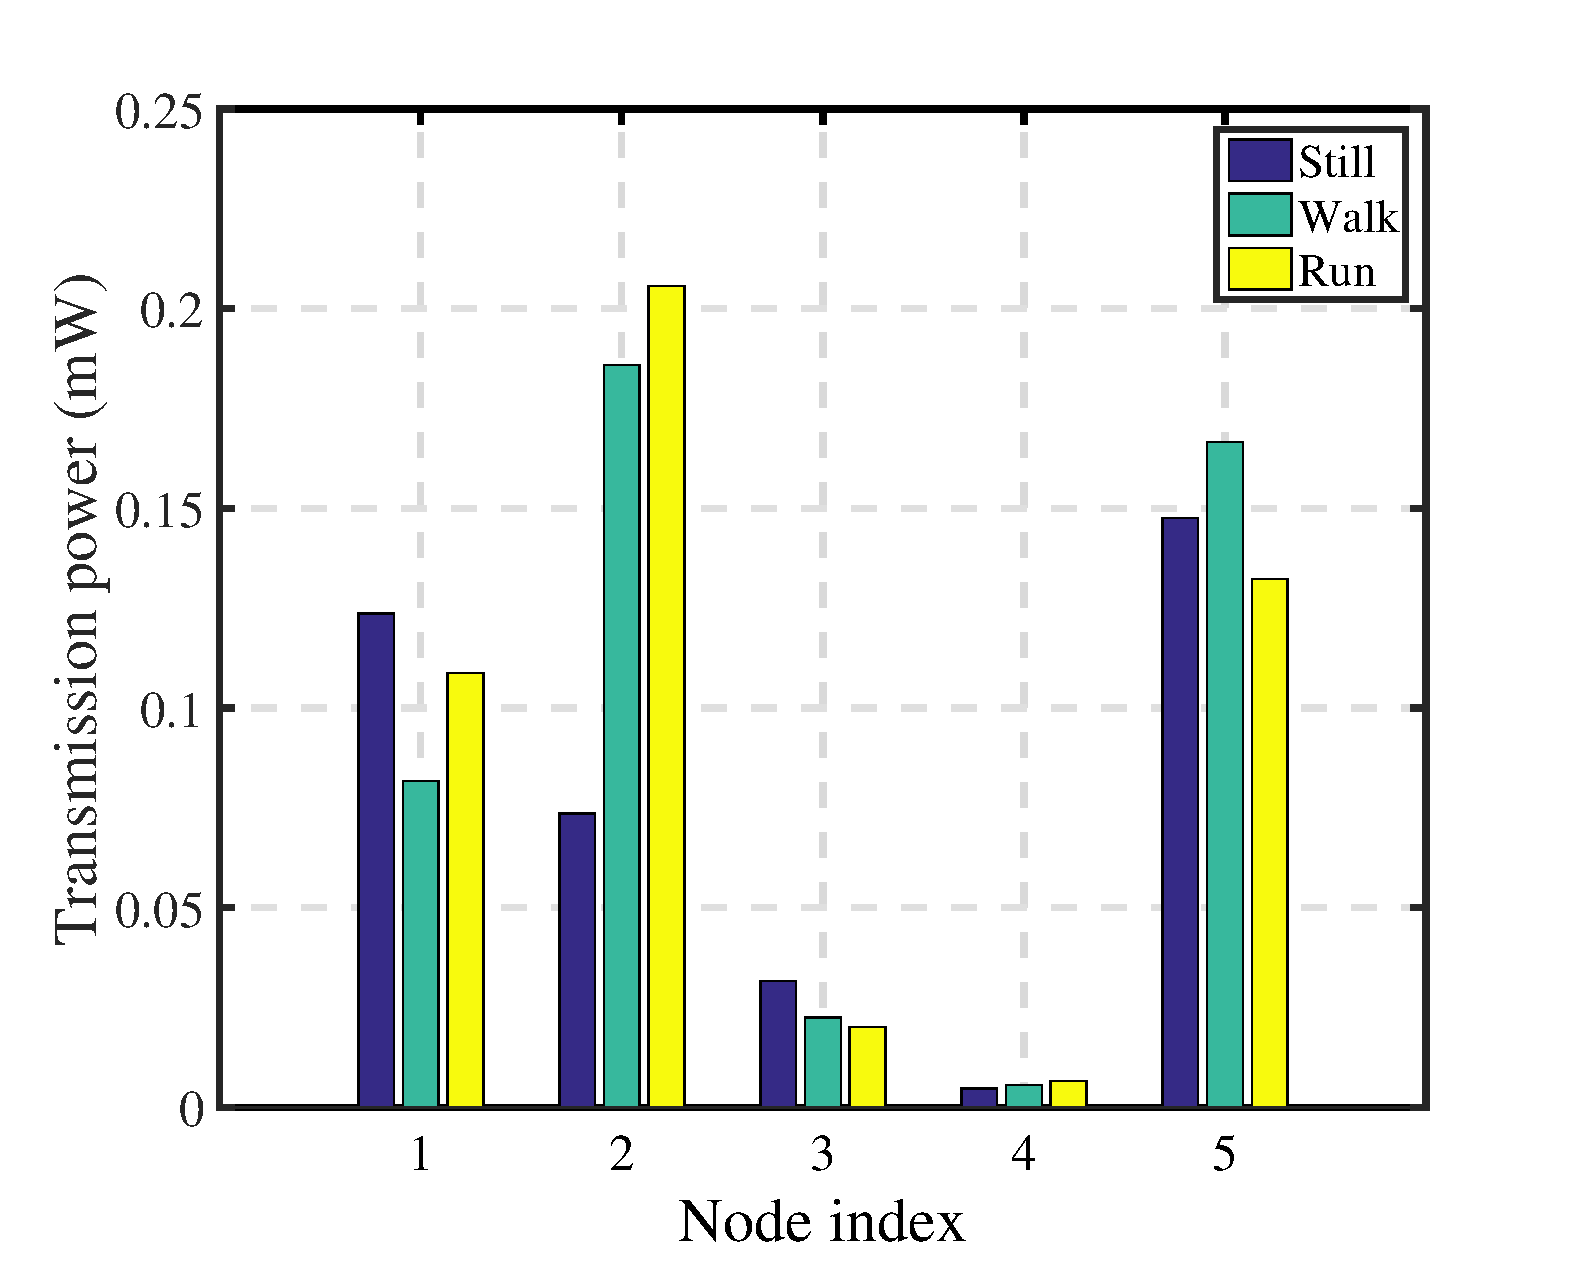
\includegraphics[width=0.22\textwidth]{PRCS_power.eps}
    }
    \hspace{0.1cm}
    \subfigure[Allocated source rate by PRCS ]{
        \label{fig:PRCS_rate}
        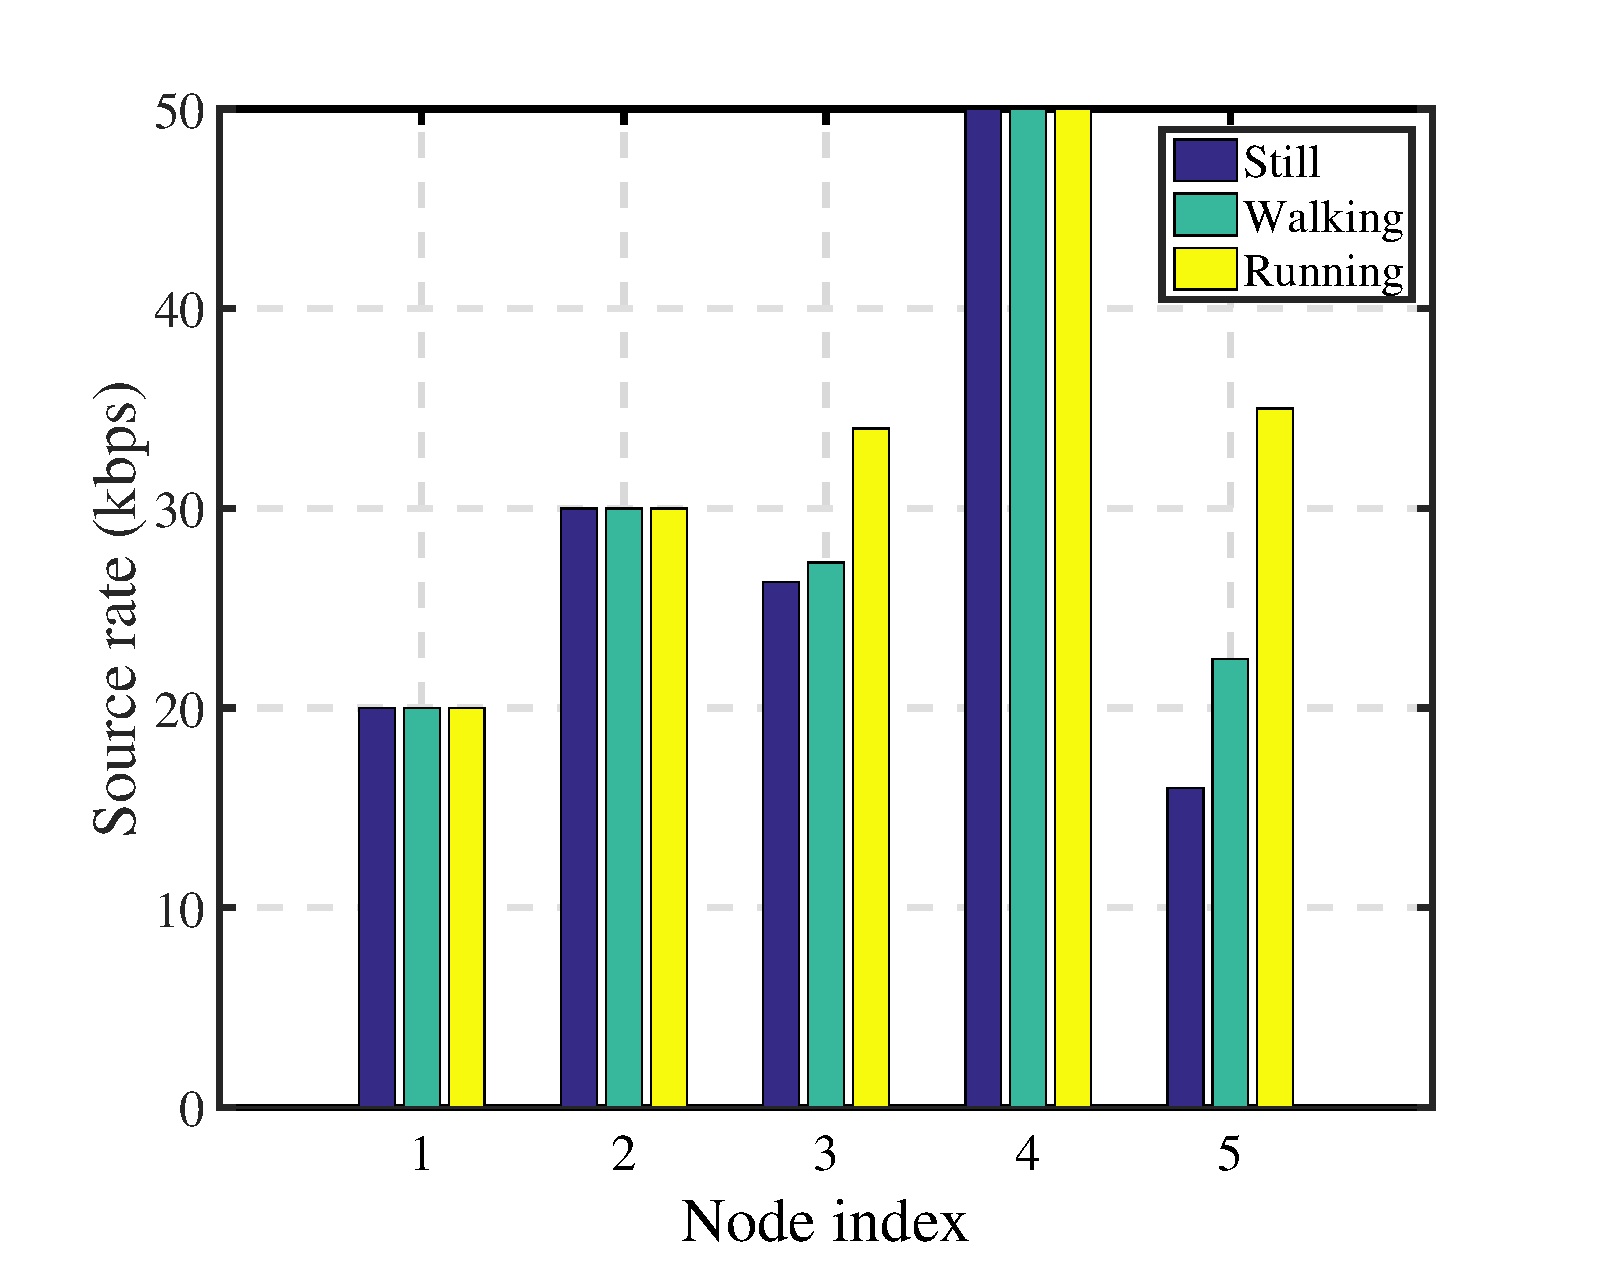
\includegraphics[width=0.22\textwidth]{PRCS_rate.eps}
    }
\caption{Allocated results for different nodes in different postures by the proposed PRCS.}
\label{fig:PRCS}
\end{figure}


\subsection{The Effectiveness of Short-term QoS Aware Slot Allocation Scheme}

Secondly, we evaluate the effectiveness of the short-term QoS aware slot allocation scheme (QASAS). Due to the time-varying EH states and the dynamic link qualities, the packet losses will occur with uncertainty. Besides, the arriving energy is also time-varying, thus the number of packets transmitted in each superframe is fluctuant, which causes that the number of the blocked packets cannot be predicted. If the blocked packets cannot be transmitted to the hub, not only the blocked packets but also the arriving packets will have a high packet delay. Furthermore, the short-term QoS performances will decrease due to the time-varying EH states.

Compared with the long-term PRCS, the short-term QASAS can give a timely response to the changes of the packet buffer state and the energy buffer state caused by the time-varying EH states. When there are many blocked packets in the packet buffer and residual energy in the energy buffer, more slots will be allocated for transmitting the blocked packets based on the level of the residual energy. Without using the QASAS, the number of packets keeps at a high level due to the time-varying EH states as shown in Fig. \ref{fig:cp_packets_without_slot}.
Fortunately, the QASAS can timely transmit the blocked packets based on the packet buffer state and the energy buffer state. Hence, the number of the packet buffer can stay a low level as shown in Fig. \ref{fig:cp_packets_with_slot}.
Therefore, the timely response to the block packets caused by the time-varying EH states can improve the short-term QoS performances.

\begin{figure}[!htb]
\centering
    \subfigure[Without using QoS Aware Slot Allocation Scheme]{
        \label{fig:cp_packets_without_slot}
        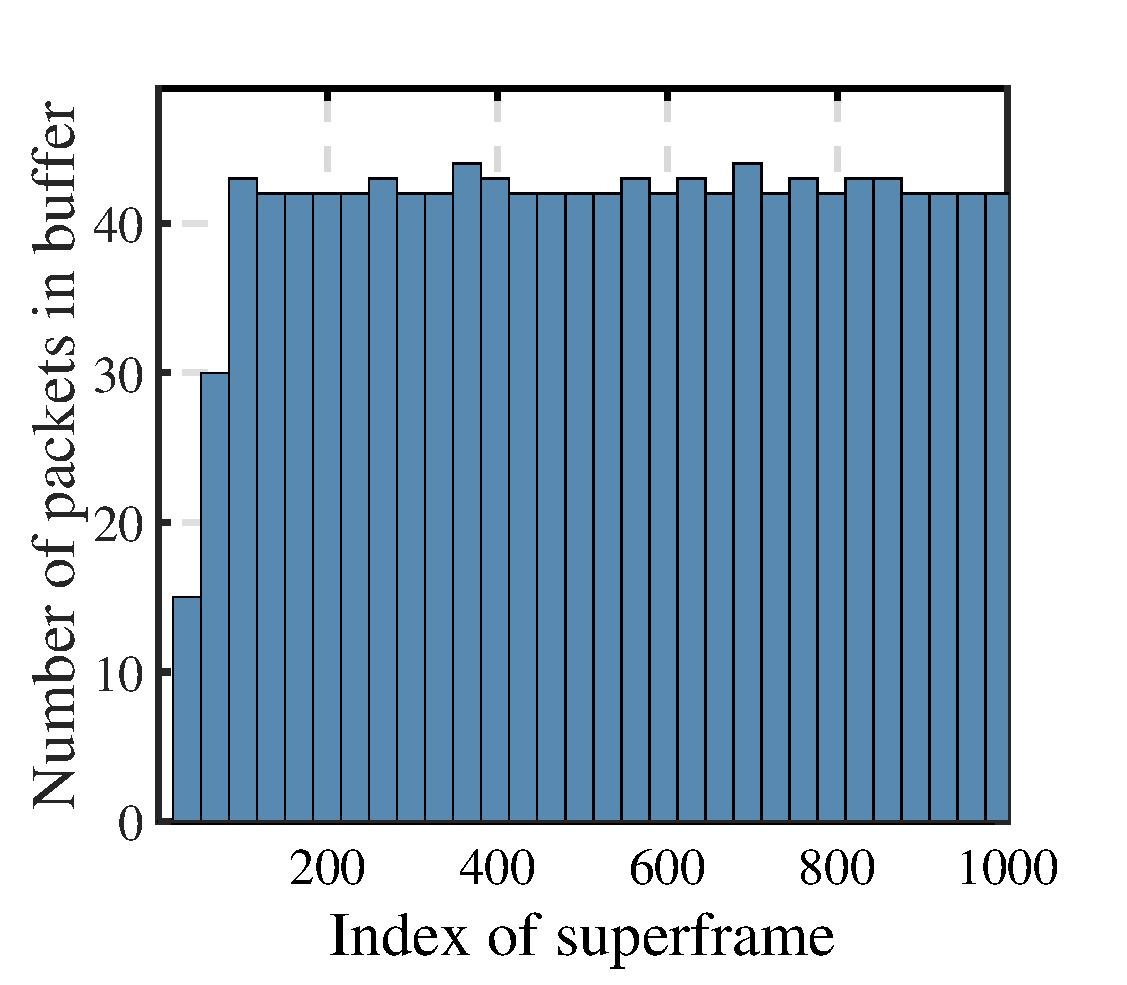
\includegraphics[width=0.22\textwidth]{cp_packets_without_slot.eps}
    }
    \hspace{-0.1cm}
    \subfigure[With using QoS Aware Slot Allocation Scheme ]{
        \label{fig:cp_packets_with_slot}
        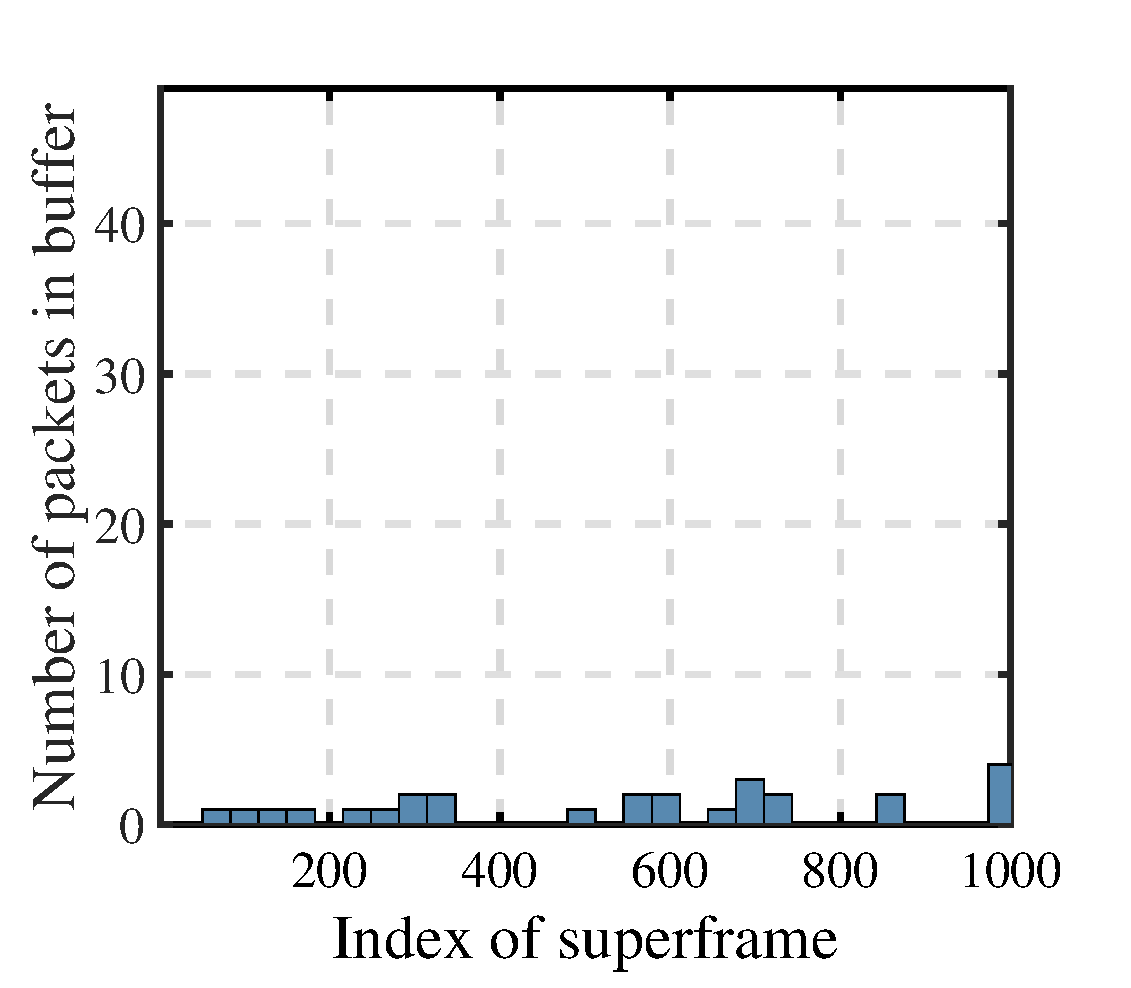
\includegraphics[width=0.22\textwidth]{cp_packets_with_slot.eps}
    }
\caption{Number of packets in the buffer of node 4 changes before and after adopting the QoS Aware Slot Allocation Scheme (QASAS).}
\label{fig:cp_Packets}
\end{figure}


\subsection{The Influence of Different Mean of Shadowing on Performance}
%\subsection{Simulation Results of Power-Rate-Slot Control Schemes}
For better evaluating the effectiveness of the long-term power-rate control scheme and the short-term slot allocation scheme, we compare them with two comparison schemes: the offline scheme \cite{huang2014optimal} and the online scheme \cite{ibarra2016qos} in terms of the average PLR, packet delay, throughput and energy per bit. For simulating the impact of the changes in the environment on the QoS performances, the mean of the shadowing can be adjusted to change the statistical characterizations of the wireless channel. The higher mean of the shadowing represents the worse link quality of the wireless channel. In this paper, we assume the means of the shadowing for all nodes have the same change when the environment condition changes, and study the influence of the mean of the shadowing on the QoS performances. 

As shown in Fig. \ref{fig:cp_PLR} and Fig. \ref{fig:cp_delay}, the proposed PRS-RA scheme obtains the lowest PLR performance and the lowest packet delay which satisfying the QoS requirements, even comparing with the offline scheme. 
This is because the proposed PRS-RA scheme explores the time-varying and heterogeneous EH states to dynamically adjust the allocation of the source rate, the transmission power and the slots for each node. Firstly, the statistical characterizations of the EH states are utilized to adjust the transmission power for maximizing the throughput with the satisfaction of the long-term QoS performances. Then, the real-time EH states of each node are investigated to dynamically allocate the time slots for timely transmitting the blocked packets, which can reduce both the packet delay and the average PLR. In Fig. \ref{fig:cp_energyPerBit}, the energy cost per bit of the proposed PRS-RA is closer to that of the offline scheme, which optimally adjusts the transmission power in real-time based on the real-time path loss of the channel with the priori knowledge of the channel states and EH states. The energy efficiency of the proposed PRS-RA is much better than that of the online scheme with only the statistical information of channel state and the EH states. This is because the transmission power in the proposed PRS-RA is first allocated to support the long-term QoS performances based on the EH states, and the effective slot allocation can further guarantee there is enough power to transmit the data packets in the allocated slots, which can avoid the waste of energy due to the packet losses. In addition, the energy efficiency of all schemes increases with the mean of the shadowing. This is because much larger transmission power is needed to cope with the worse link quality.


As for the throughput in Fig. \ref{fig:cp_Throughput}, the throughput of the proposed PRS-RA scheme decreases with the mean of the shadowing. When the link quality becomes worse with a higher mean of the shadowing, the long-term power-rate control scheme (PRCS) dynamically adjust the transmission rate and the source rate based on the link quality. Generally, the transmission power will be increased to guarantee the QoS performances and the source rate will be decreased to ensure the integrity of data with a lower PLR. In addition, the short-term QoS aware slot allocation scheme (QASAS) dynamically analyzes the states of each node and then optimizes the appropriate slots to cope with the blocked packets in the buffer. Hence, the bandwidth utilization of the proposed PRA-SA reaches to 94\%, which is higher than the online scheme, thus more channel resource can be utilized by other WBANs.


\begin{figure*}[!htb]
\centering
    \subfigure[Average PLR]{
        \label{fig:cp_PLR}
        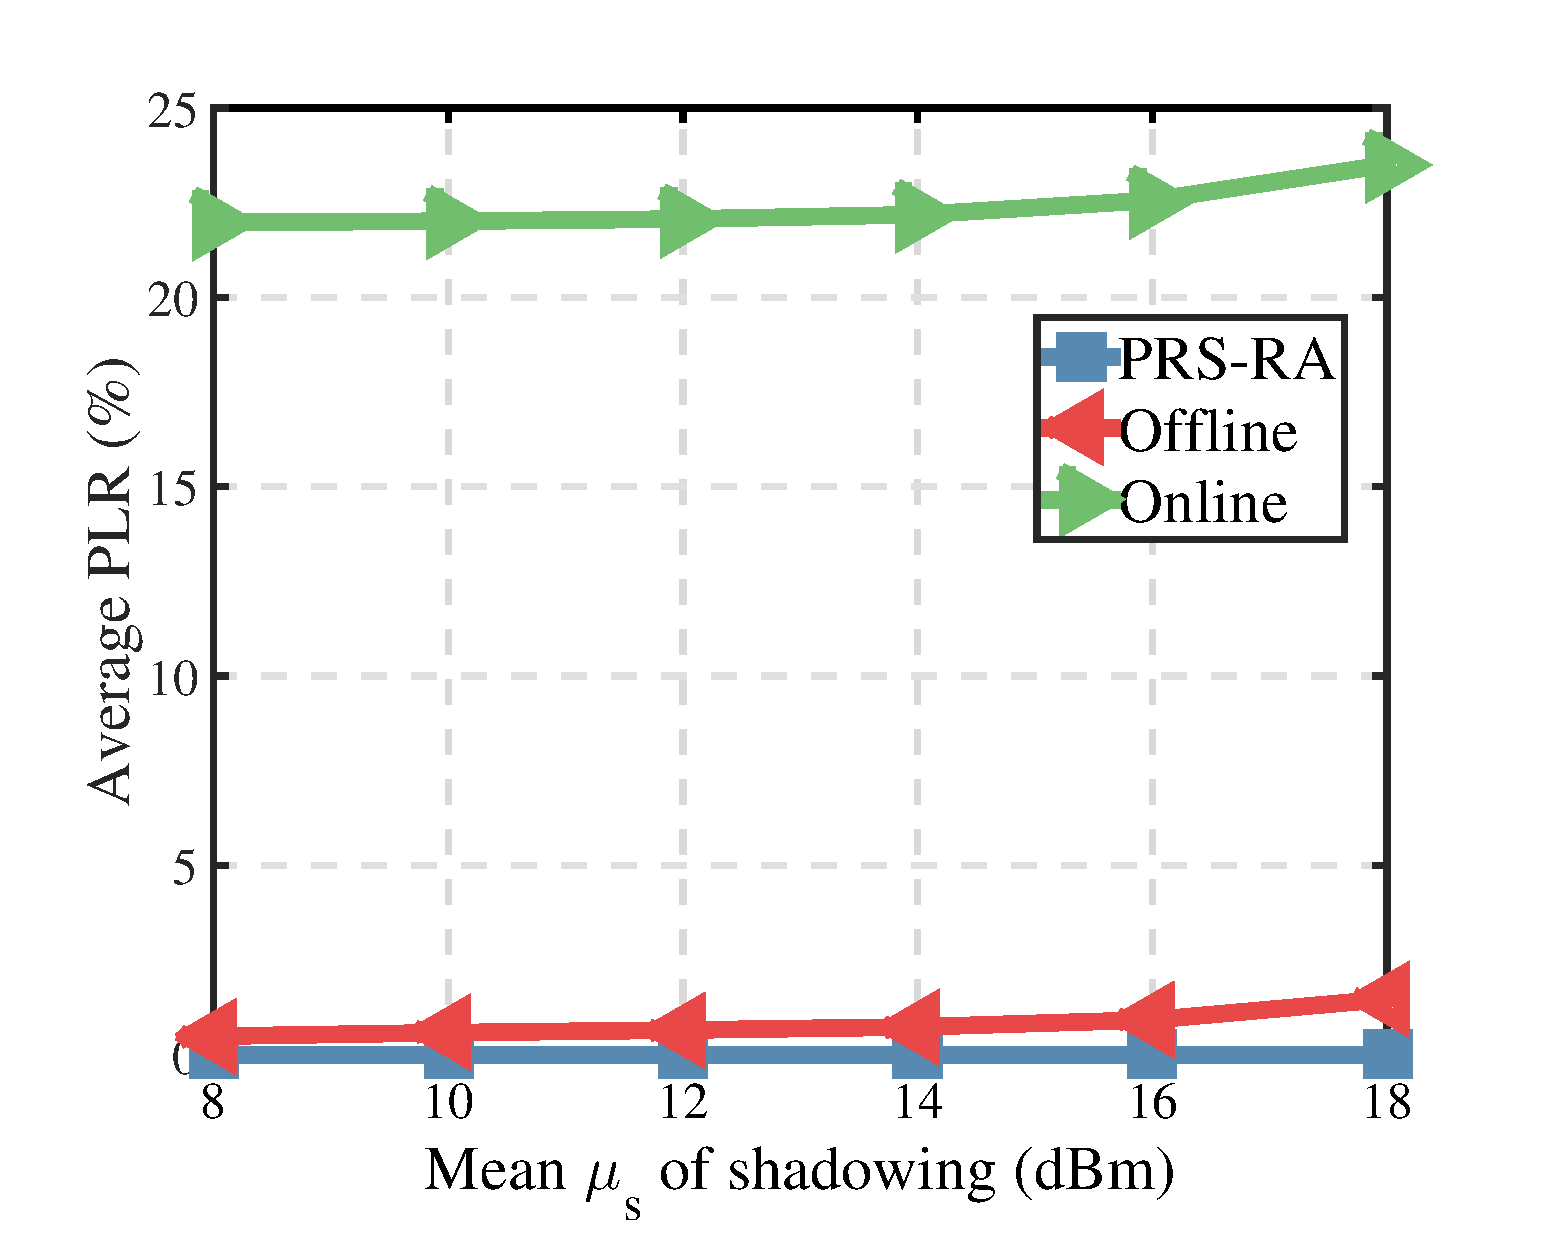
\includegraphics[width=0.3\textwidth]{cp_PLR.eps}
    }
    \hspace{-0.6cm}
    \subfigure[Packet delay]{
        \label{fig:cp_delay}
        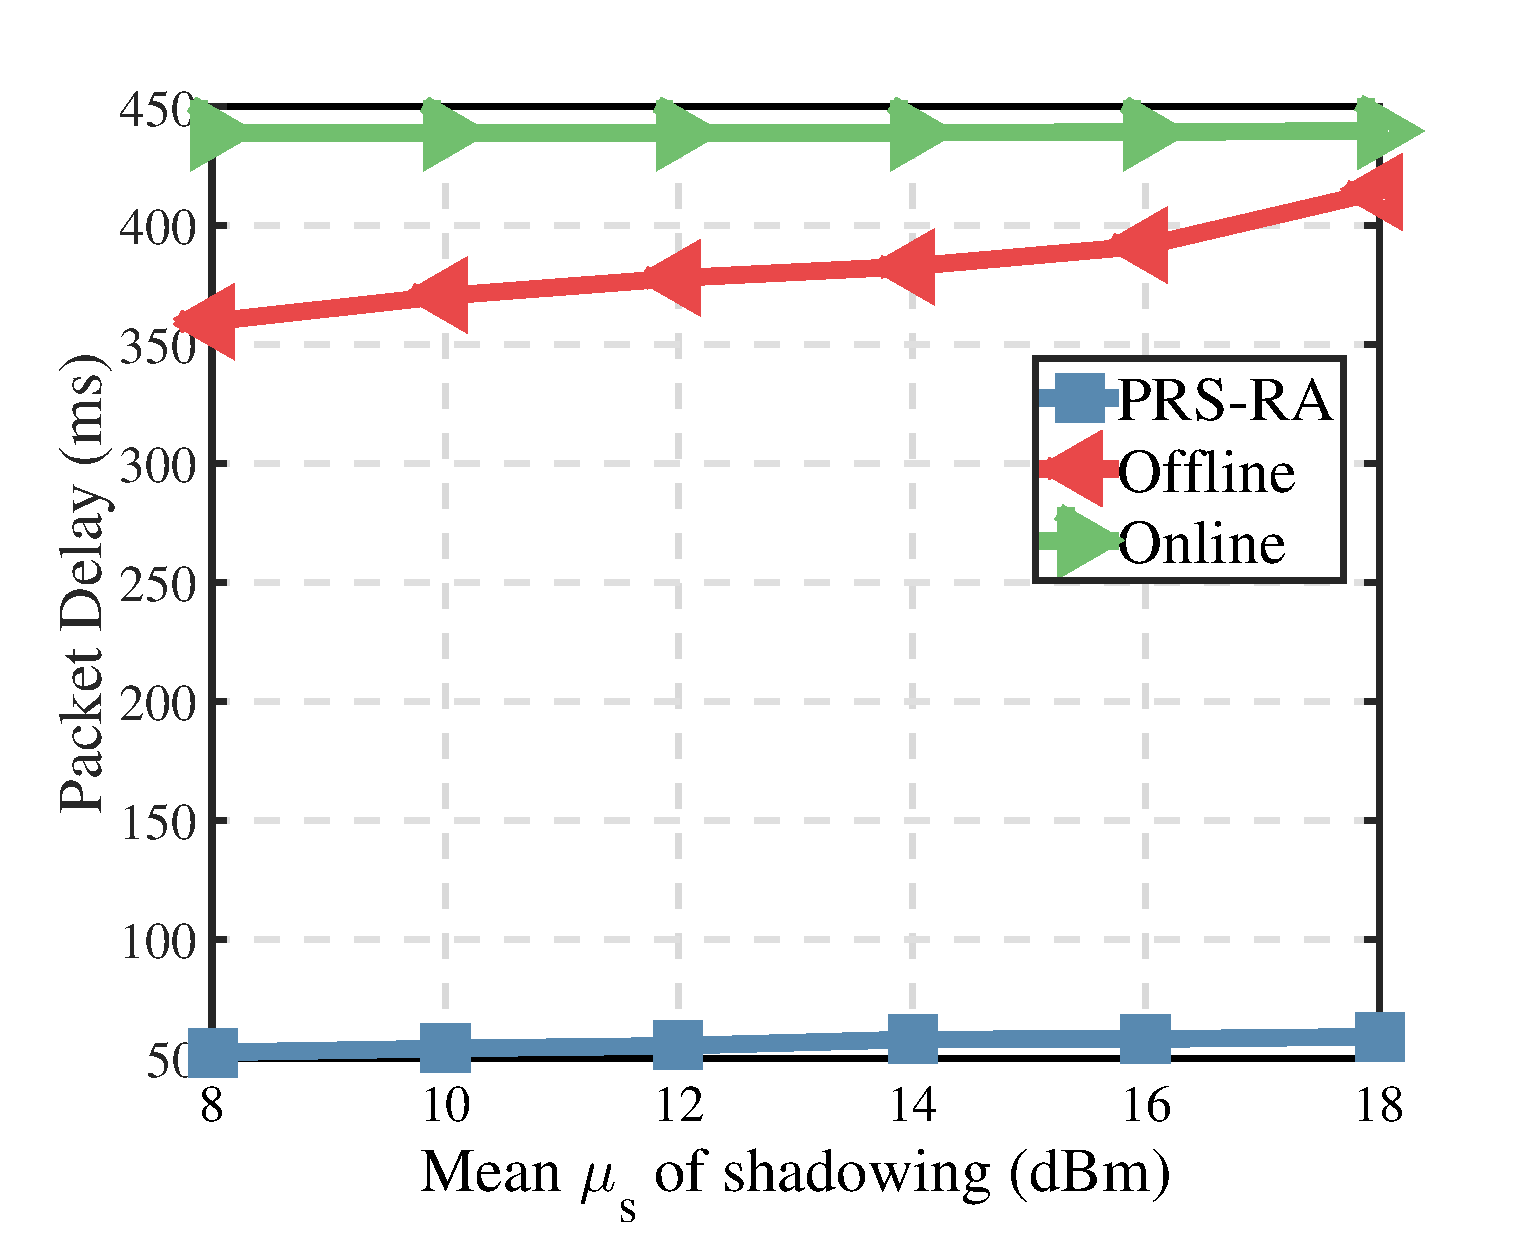
\includegraphics[width=0.3\textwidth]{cp_Delay.eps}
    }
		\hspace{-0.6cm}
    \subfigure[Energy cost per bit]{
        \label{fig:cp_energyPerBit}
        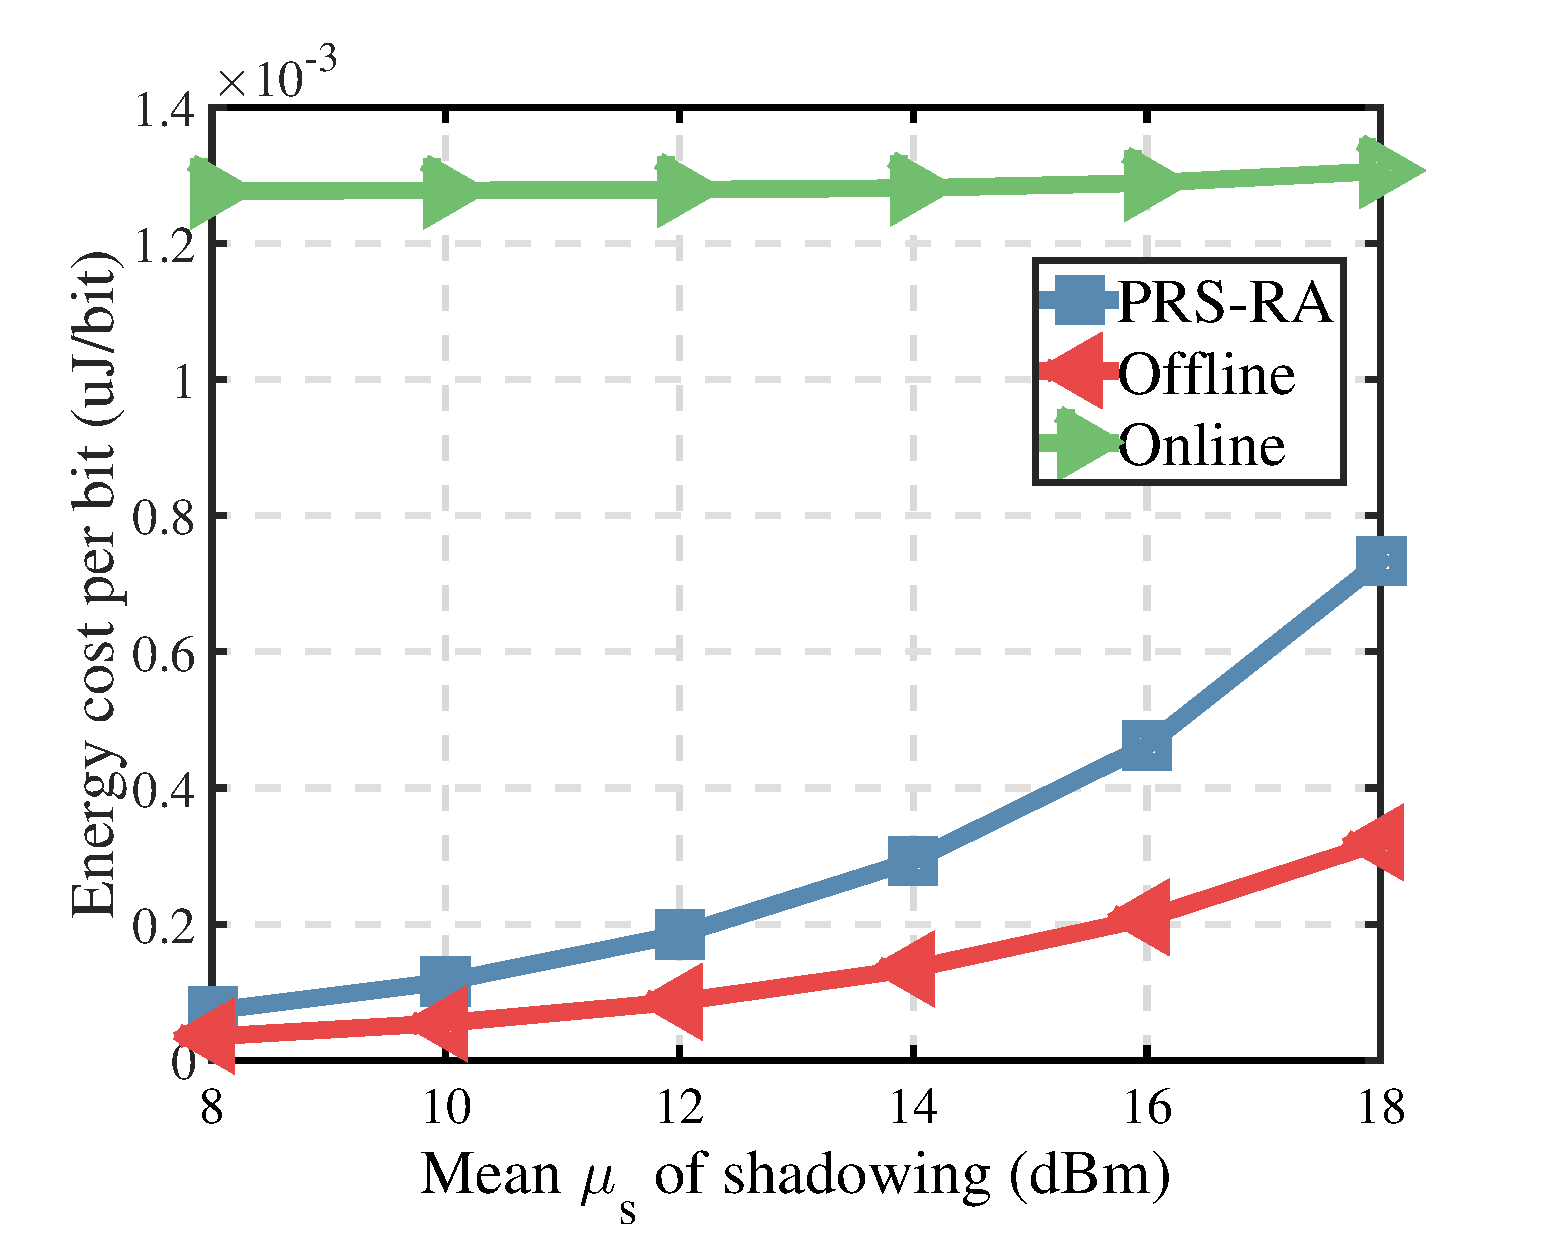
\includegraphics[width=0.3\textwidth]{cp_energyPerBit.eps}
    }
		\hspace{-0.6cm}
    \subfigure[Throughput]{
        \label{fig:cp_Throughput}
        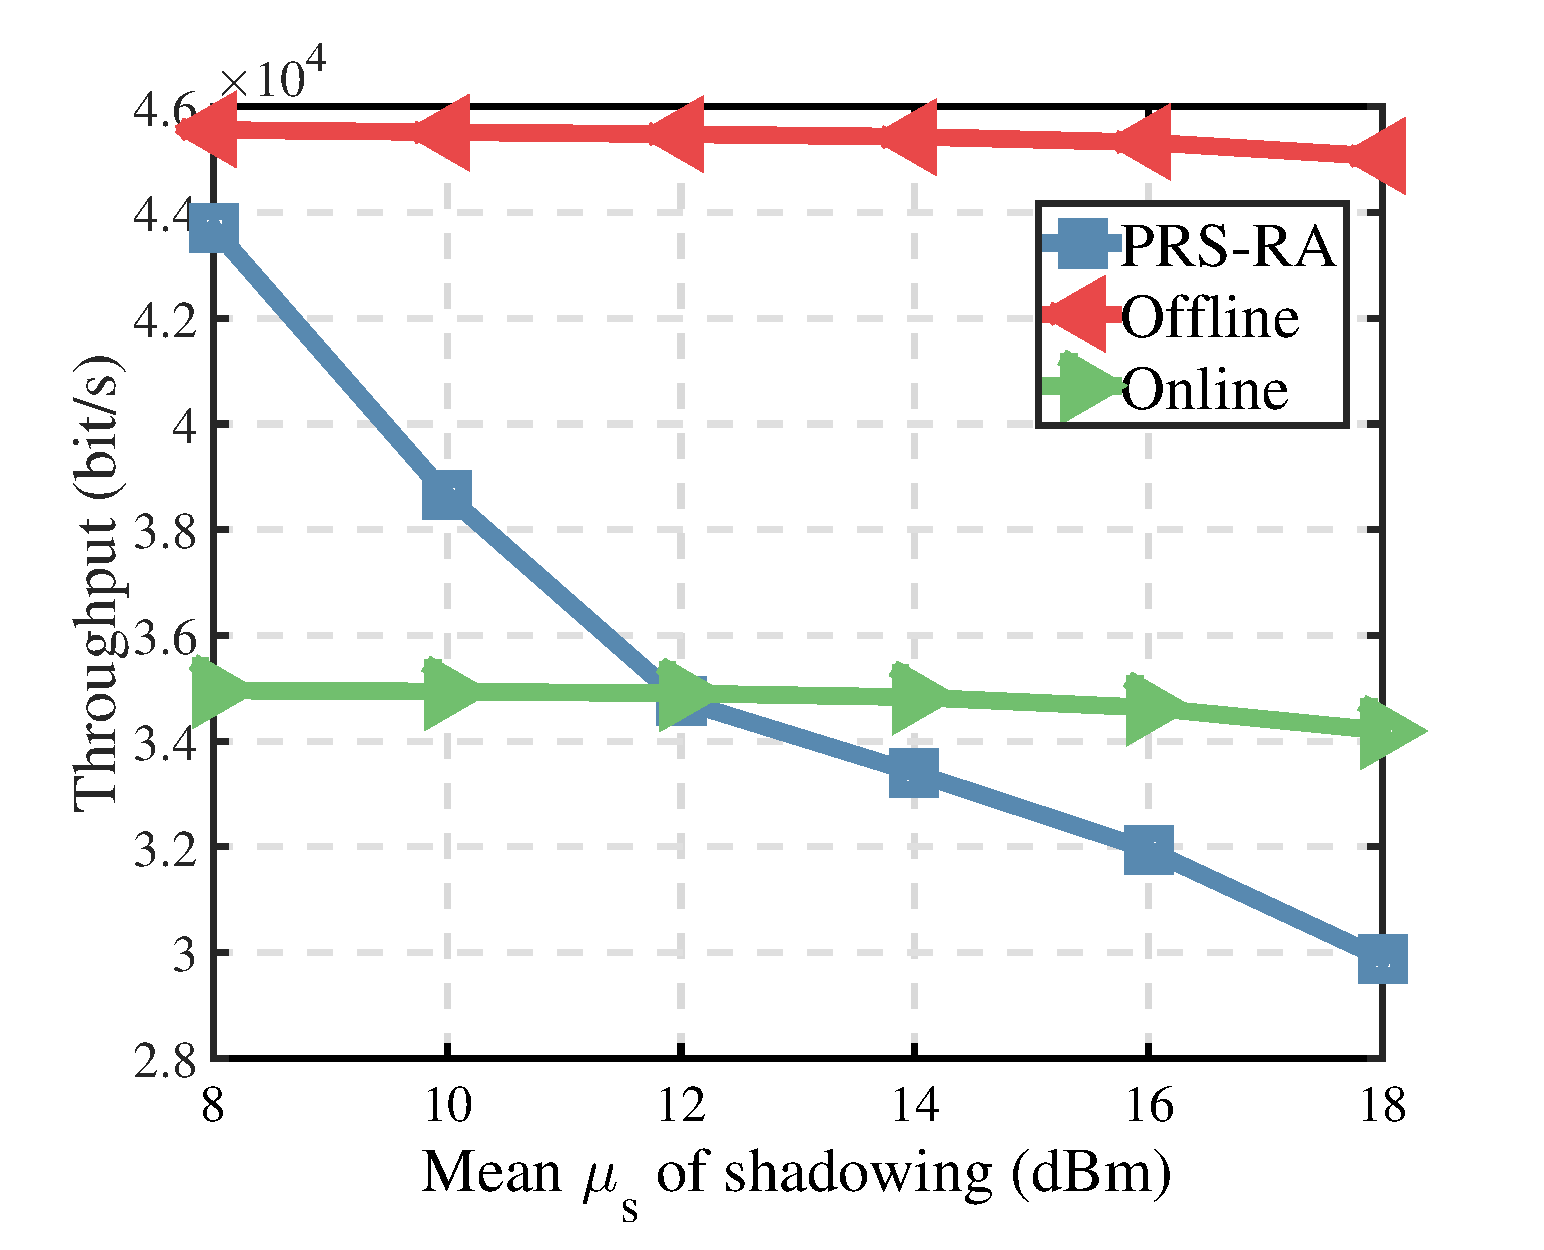
\includegraphics[width=0.3\textwidth]{cp_Throughput.eps}
    }
		\hspace{-0.6cm}
    \subfigure[Bandwidth utilization]{
        \label{fig:cp_bandwidth}
        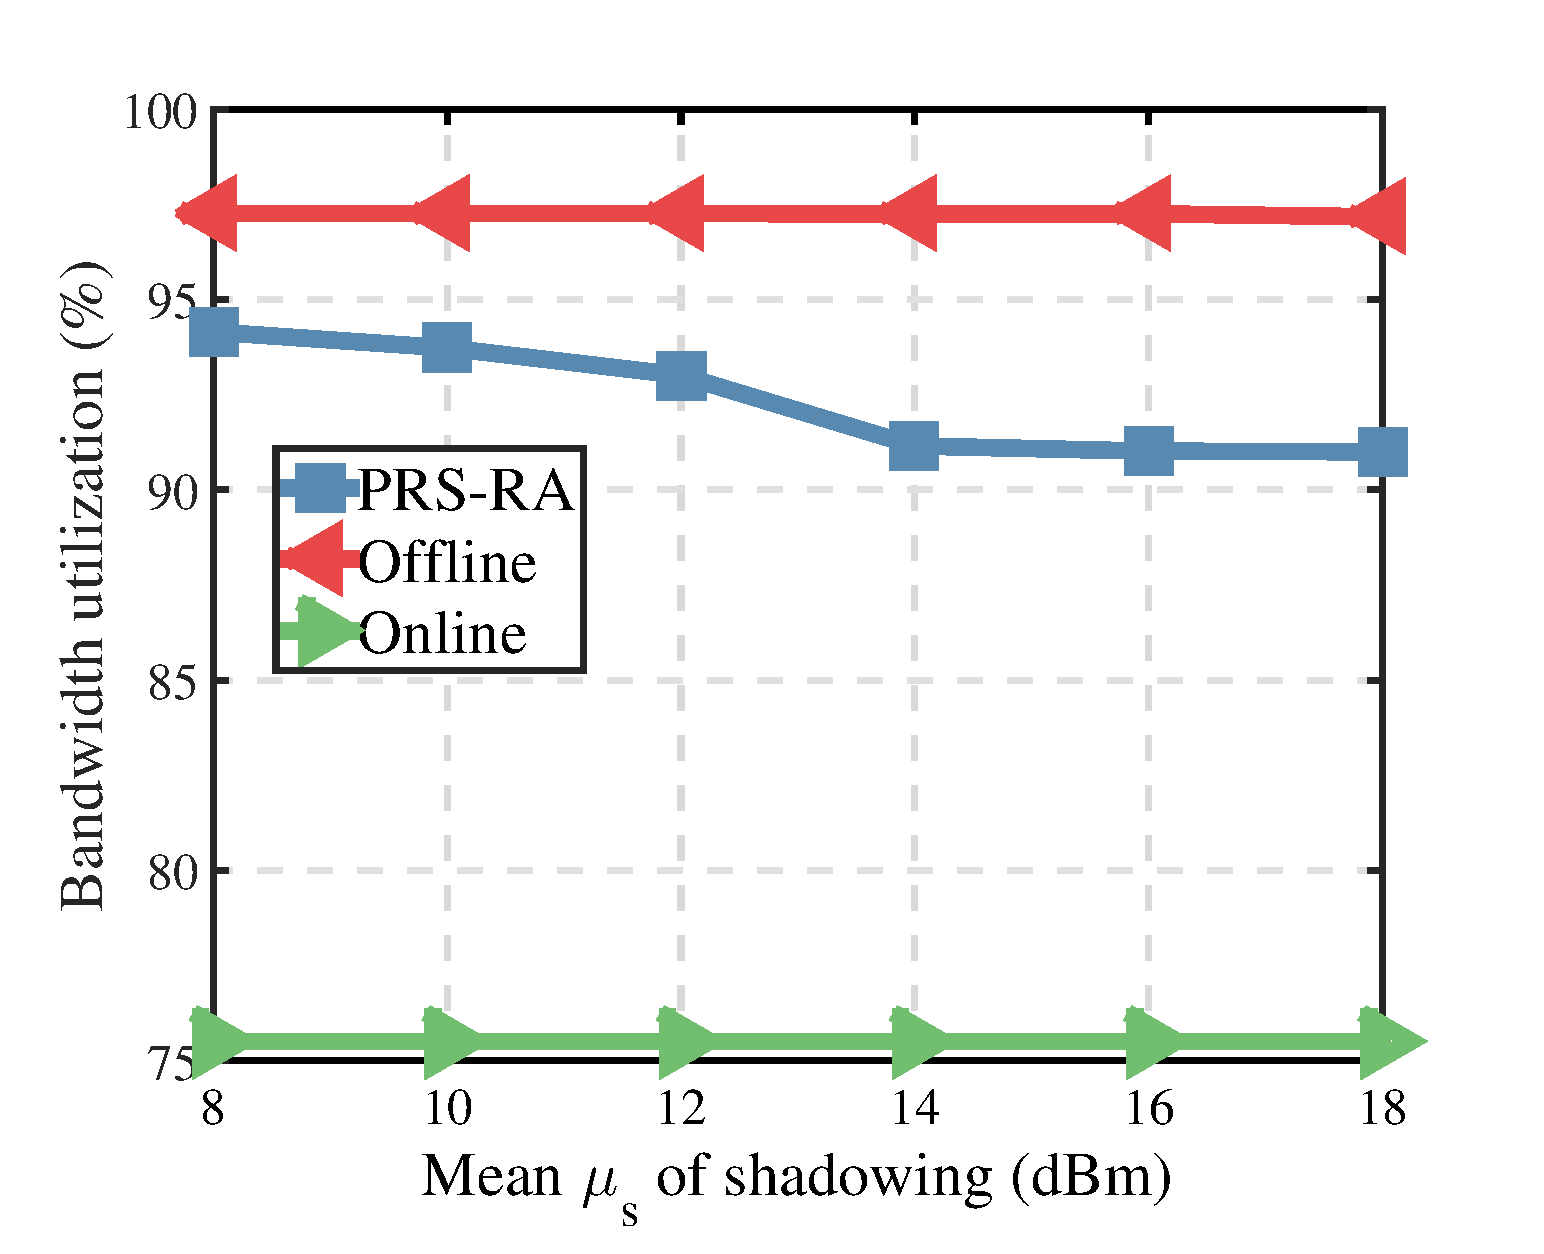
\includegraphics[width=0.3\textwidth]{cp_bandwidth.eps}
    }
\caption{The QoS performances of different algorithms.}
\label{fig:cp_QoS}
\end{figure*}



\begin{figure}[!htb]
\centering
    \subfigure[Average PLR performance]{
        \label{fig:EHefficiency_PLR}
        \includegraphics[width=0.22\textwidth]{EHefficiency_PLR.eps}
    }
    \hspace{-0.1cm}
    \subfigure[Packet delay performance ]{
        \label{fig:EHefficiency_Delay}
        \includegraphics[width=0.22\textwidth]{EHefficiency_Delay.eps}
    }
		\hspace{-0.1cm}
    \subfigure[Throughput performance]{
        \label{fig:EHefficiency_Throughput}
        \includegraphics[width=0.22\textwidth]{EHefficiency_Throughput.eps}
    }
		\hspace{-0.1cm}
    \subfigure[Bandwidth utilization performance]{
        \label{fig:EHefficiency_bandwidth}
        \includegraphics[width=0.22\textwidth]{EHefficiency_bandwidth.eps}
    }
\caption{QoS performances versus the EH efficiency ratio.}
\label{fig:cp_EHefficiency}
\end{figure}

\subsection{The Influence of Different EH Efficiencies on Performance}
To evaluate the effectiveness of the long-term power-rate control scheme (PRCS) and the short-term QoS aware slot allocation scheme (QASAS) separately, we compare three different schemes: 1) the proposed PRS-RA with both PRCS and QASAS, 2) the proposed PRS-RA with PRCS, 3) the proposed PRS-RA with QASAS. 
The statistical characterizations of the EH decide how much energy can be collected for each node, which has a great effect on the achievable QoS performances of these schemes. Thus, we gradually change the energy acquisition rate $\rho$ by multiplying an EH efficiency ratio $\lambda$, and the final energy acquisition rate is expressed as $\lambda \cdot \rho$. The smaller EH efficiency ratio $\lambda$ means energy harvester can collect less energy when the energy harvester stays the ON state. The QoS performances versus the EH efficiency ratio are given in Fig. \ref{fig:cp_EHefficiency}.

As shown in Fig. \ref{fig:EHefficiency_PLR} and Fig. \ref{fig:EHefficiency_Delay}, the higher efficiency ratio means that the nodes can collect more energy to transmit the packets better, thus both of the average PLR and packet delay decrease with the EH efficiency ratio. So the throughput and the bandwidth utilization are improved correspondingly with more harvesting energy, as shown in Fig. \ref{fig:EHefficiency_Throughput} and Fig. \ref{fig:EHefficiency_bandwidth}.

Comparing with the proposed PRS-RA with QASAS, the PRS-RA with PRCS has the better PLR and delay performance in Fig. \ref{fig:EHefficiency_PLR} and Fig. \ref{fig:EHefficiency_Delay}, while the throughput and the bandwidth utilization performance of the PRS-RA with QASAS are much better than those of the PRS-RA with PRCS in Fig. \ref{fig:EHefficiency_Throughput} and Fig. \ref{fig:EHefficiency_bandwidth}. This is because the PRS-RA with PRCS optimally allocates the transmission power and the source rate to support the long-term QoS performances based on the statistical characteristics of the EH states, hence the average PLR and packet delay can be guaranteed. Besides, the PRS-RA with QASAS firstly evaluates the sensor state according to the real-time EH states and the packet buffer states. And it dynamically adjusts the allocation of the slots for each node based on the sensor state. The real-time slot allocation can give a timely response to the changes of the EH states and the packet buffer, and the bandwidth utilization and the throughput performance can be improved with the real-time slot allocation.
In addition, because both the long-term QoS and short-term QoS performances are taken full consideration in the proposed PRS-RA with both PRCS and the QASAS, the proposed PRS-RA with both PRCS and QASAS achieves the best PLR and packet delay performance with exploring the time-varying EH states in Fig. \ref{fig:EHefficiency_PLR} and Fig. \ref{fig:EHefficiency_Delay}, while the throughput and bandwidth utilization performance are between those of the PRS-RA with PRCS and the PRS-RA with QASAS in Fig. \ref{fig:EHefficiency_Throughput} and Fig. \ref{fig:EHefficiency_bandwidth}.


\renewcommand\arraystretch{1.2}


\section{Conclusion} \label{sec:conclusion}
In this paper, we optimize the resource allocations to improve both the long-term QoS and the short-term QoS performances in the EH-powered WBAN system, while the time-varying and heterogeneous EH states are fully taken into consideration. Firstly, we design a joint Power-Rate control scheme (PRCS) in terms of the transmission power and the source rate to ensure the long-term QoS performances based on both the EH states and the dynamic link quality. Secondly, we evaluate the node state in real time based on the packet buffer state and the energy buffer state, and then a QoS aware slot allocation scheme is adopted to dynamically allocate the slots based on the node states for timely transmitting the blocked packets in the buffer. The simulation results demonstrate that the joint Power-Rate control
scheme (PRCS) can effectively improve the long-term QoS performances in terms of PLR, delay and throughput. In addition, the short-term QoS aware slot allocation scheme (QASAS) can timely allocate the slots to transmit the blocked packets, thus the QoS performances are further improved by adopting both PRCS and QASAS.


% use section* for acknowledgment
\section*{Acknowledgment}
%%%The authors sincerely thank the anonymous referees for their invaluable suggestions that have led to the present improved version of the original manuscript. This work is supported in part by the National Natural Science Foundation of China under Grant No.61671420, No.61672484, No. 61379129, and the Fundamental Research Funds for the Central Universities.
% Can use something like this to put references on a page
% by themselves when using endfloat and the captionsoff option.
\ifCLASSOPTIONcaptionsoff
  \newpage
\fi
% trigger a \newpage just before the given reference
% number - used to balance the columns on the last page
% adjust value as needed - may need to be readjusted if
% the document is modified later
%\IEEEtriggeratref{8}
% The "triggered" command can be changed if desired:
%\IEEEtriggercmd{\enlargethispage{-5in}}

% references section

% can use a bibliography generated by BibTeX as a .bbl file
% BibTeX documentation can be easily obtained at:
% http://mirror.ctan.org/biblio/bibtex/contrib/doc/
% The IEEEtran BibTeX style support page is at:
% http://www.michaelshell.org/tex/ieeetran/bibtex/
%\bibliographystyle{IEEEtran}
% argument is your BibTeX string definitions and bibliography database(s)
%\bibliography{IEEEabrv,../bib/paper}
%
% <OR> manually copy in the resultant .bbl file
% set second argument of \begin to the number of references
% (used to reserve space for the reference number labels box)
{
%\scriptsize
\footnotesize
%\small
\renewcommand\bibname{References}
\bibliographystyle{ieeetr}
\bibliography{energy_harvesting}
}

% biography section
%
% If you have an EPS/PDF photo (graphicx package needed) extra braces are
% needed around the contents of the optional argument to biography to prevent
% the LaTeX parser from getting confused when it sees the complicated
% \includegraphics command within an optional argument. (You could create
% your own custom macro containing the \includegraphics command to make things
% simpler here.)
%\begin{IEEEbiography}[{\includegraphics[width=1in,height=1.25in,clip,keepaspectratio]{mshell}}]{Michael Shell}
% or if you just want to reserve a space for a photo:
\newpage
\begin{IEEEbiography}[{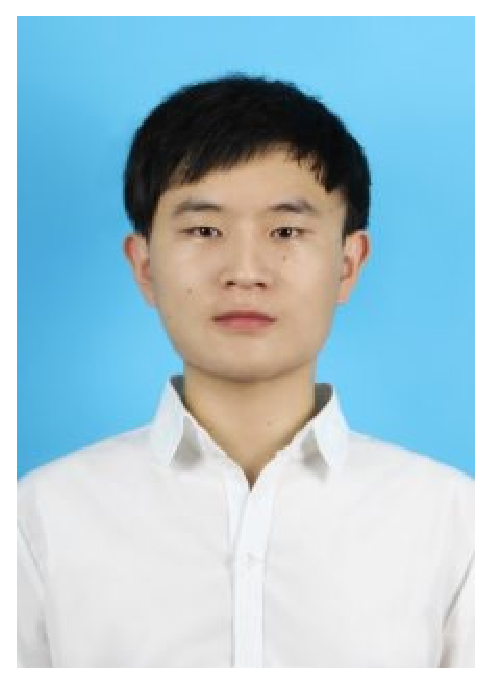
\includegraphics[width=1in,height=1.25in,clip,keepaspectratio]{ZhiqiangLiu.eps}}]{Zhiqiang Liu}
received the B.S degrees in electrical engineering from University of Science and Technology of China, Hefei, Anhui, China, in 2013, and he is currently pursuing the Ph.D. degree in electrical engineering from University of Science and Technology of China. His research interests lie resource allocation, energy-saving and Quality of Service guarantee in wireless body area networks. 
\end{IEEEbiography}%
\vspace{-20em}
\begin{IEEEbiography}[{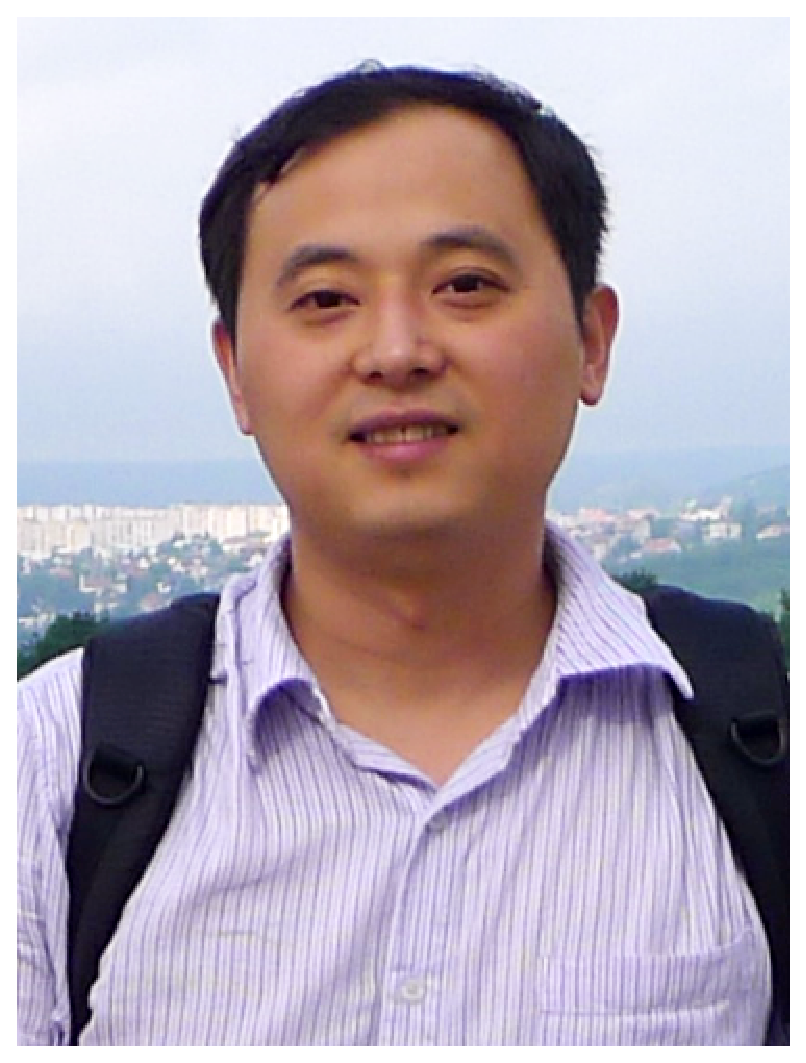
\includegraphics[width=1in,height=1.25in,clip,keepaspectratio]{BinLiu.eps}}]{Bin Liu}
received the B.S. and M.S. degrees, both in electrical engineering, from University of Science and Technology of China, Hefei, Anhui, China, in 1998 and 2001, respectively, and the Ph.D. degree in electrical engineering from Syracuse University, Syracuse, NY, in 2006. Currently, he is an Associate Professor with the School of Information Science and Technology, University of Science and Technology of China. His research interests are signal processing and communications in wireless sensor and body area networks.
\end{IEEEbiography}%
\vspace{-20em}
\begin{IEEEbiography}[{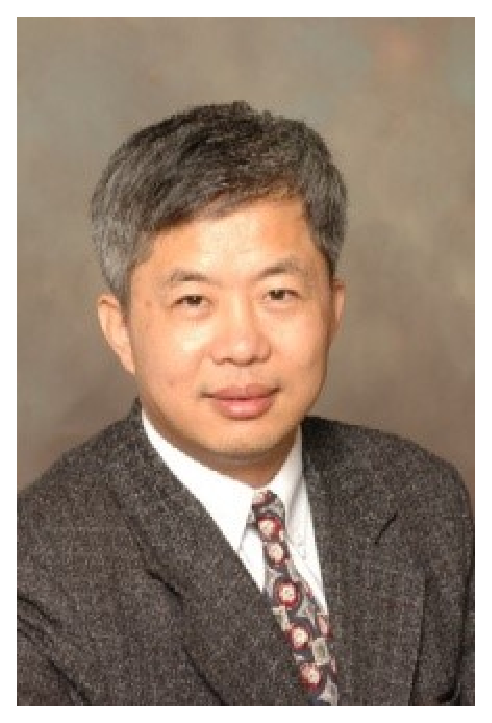
\includegraphics[width=1in,height=1.25in,clip,keepaspectratio]{ChangwenChen.eps}}]{Chang Wen Chen}
   (F'04) is a Professor of Computer Science and Engineering at the State University of New York at Buffalo, USA. Previously, he was Allen S. Henry Endowed Chair Professor at Florida Institute of Technology from 2003 to 2007, a faculty member at the University of Missouri - Columbia from 1996 to 2003 and at the University of Rochester, Rochester, NY, from 1992 to 1996. He has been the Editor-in-Chief for IEEE Trans. Multimedia since 2014. He has also served as the Editor-in-Chief for IEEE Trans. Circuits and Systems for Video Technology from January 2006 to December 2009 and an Editor for Proceedings of IEEE, IEEE TMM, IEEE JSAC, IEEE JETCAS, and IEEE Multimedia Magazine. He and his students have received eight (8) Best Paper Awards or Best Student Paper Awards and have been placed among Best Paper Award finalists many times. He is a recipient of Sigma Xi Excellence in Graduate Research Mentoring Award in 2003, Alexander von Humboldt Research Award in 2009, and SUNY-Buffalo Exceptional Scholar - Sustained Achievements Award in 2012. He is an IEEE Fellow and an SPIE Fellow. 
\end{IEEEbiography}%
 


% You can push biographies down or up by placing
% a \vfill before or after them. The appropriate
% use of \vfill depends on what kind of text is
% on the last page and whether or not the columns
% are being equalized.

%\vfill

% Can be used to pull up biographies so that the bottom of the last one
% is flush with the other column.
%\enlargethispage{-5in}



% that's all folks
\end{document}


